\documentclass[10pt]{beamer}

\usepackage[utf8]{inputenc}
\usepackage{enumitem, environ, marvosym, pgfplots, siunitx, xspace}
\usetikzlibrary{arrows.meta,   	        	% big arrows
				calc,						% coordinates calculations
				decorations.markings,		% in-line arrows
				overlay-beamer-styles,		% for vsible on=<> overlays
				positioning,				% place nodes
				}
\usepgfplotslibrary{groupplots}

%% Lengths

% base unit for coordinates
\newlength\quantum
\newlength\quanta
\setlength\quantum{3pt}
\setlength\quanta{\quantum}

% slides dimensions = N * quantum,
% ratio 120/90 = 4/3, with 3 quanta
% for the footline
\setlength{\paperwidth}{120\quanta}
\setlength{\paperheight}{93\quanta}

% set a footline with total height (height + depth) of 3 quanta
\newlength\tinyxheight
\newlength\flheight
\newlength\fldepth
\settoheight{\tinyxheight}{\tiny x}
\setlength\flheight{\dimexpr 1.5\quantum + 0.5\tinyxheight \relax}
\setlength\fldepth{\dimexpr 1.5\quantum - 0.5\tinyxheight \relax}

% width of a column in a five (V) columns layout
\newlength\colv
\newlength\colvsep  % including the inter-column spacing
\setlength\colv{17.6\quanta}
\setlength\colvsep{\dimexpr\colv + \baselineskip\relax}

% big column width (two columns + one baseline skip)
\newlength\bigcol
\newlength\halfbigcol
\setlength\bigcol{\dimexpr 2\colv + \baselineskip\relax}
\setlength\halfbigcol{0.5\bigcol}

% depth in Large fonts, for positioning titles
\newlength\Largeydepth
\settodepth{\Largeydepth}{\Large y}

% M height in footnotesize fonts, for positioning tick labels
\newlength\ssMheight
\settoheight{\ssMheight}{\scriptsize M}

% temporary lengths to locally replace long length calculations
\newlength\templen
\newlength\buffer

% map layout
\newlength\w
\newlength\e

%% lists stuff
\newenvironment{listed}{
	\begin{itemize}[nosep]
	\setlength\itemsep{2\quanta}  % adds to the existing baseline skip
	}{
	\end{itemize}
	}

% remove indentation
\settowidth{\leftmargini}{\usebeamertemplate{itemize item}}
\addtolength{\leftmargini}{.36\labelsep} % narrower than usual item symbol

%% Overall style

\colorlet{col}{orange}  % main color
% map colors
\colorlet{hls1}{black}
\colorlet{hls2}{black}
\colorlet{hls3}{black}

% square bullet items
\setbeamertemplate{itemize item}[square]
\setbeamercolor{itemize item}{fg=col}

% enumitem overrides beamer settings,
% so list styles have to be re-specified
\setitemize{label=\usebeamerfont*{itemize item}%
  \usebeamercolor[fg]{itemize item}
  \usebeamertemplate{itemize item}}



%% TikZ based slide template

% slide environment composed of a TikZ picture
% with the following nodes
%
% (NW) ----- (N) ----- (NE)
%   |         |         |
%   |         |         |
%  (W) ----- (C) ----- (E)
%   |         |         |
%   |         |         |
% (SW) ----- (S) ----- (SE)

\NewEnviron{slide}[1][]{%
\begin{frame}[t]%
	\makebox[\textwidth][c]{%
		\begin{tikzpicture}[overlay, remember picture, inner sep=0pt]%
		
		\node (N) at (page cs:0,45) {};
		\node (S) at (page cs:0,-45) {};
		\node (W) at (page cs:-60,0) {};
		\node (E) at (page cs:60,0) {};
		\node (NW) at (page cs:-60,45) {};
		\node (NE) at (page cs:60,45) {};
		\node (SW) at (page cs:-60,-45) {};
		\node (SE) at (page cs:60,-45) {};
		\node (C) at (page cs:0,0) {};
		
		\node[anchor=north west, align=left, font=\Large, black!80,
			  yshift=\Largeydepth+.95pt, xshift=-.95pt] (title)
			at (page cs:-52,37) {#1};
			
			\normalsize\BODY
		
		\end{tikzpicture}}%
\end{frame}}

% draw help lines
\newcommand\drawhelplines{
	% title top lines
	\draw[teal] (page cs:-60,37) -- (page cs:60,37)
				(page cs:-60,31) -- (page cs:60,31);
	% pictures grid
	\draw[gray] foreach \c in {0,...,4}{
				(p5cl cs:\c,0)  -- (p5cl cs:\c,15)
				(p5cr cs:\c,0)  -- (p5cr cs:\c,15)
					foreach \l in {0,...,15}{
						(p5cl cs:\c,\l)  -- (p5cr cs:\c,\l)}};
	% text grid
	\draw[teal] foreach \c in {0,...,4}{
					foreach \l in {0,...,14}{
						(t5cl cs:\c,\l)  -- (t5cr cs:\c,\l)}};
	% margin
	\draw[col] (p5cr cs:1,-2) node (x) {} -- (x |- N);}

% draw full grid
\newcommand\drawfullgrid{
	\draw[gray] foreach \x in {-60,...,60}{
					(page cs:\x,-45) -- (page cs:\x,45)}
				foreach \y in {-45,...,45}{
					(page cs:-60,\y) -- (page cs:60,\y)};}



% Environment for map and title page
\NewEnviron{maplayout}{

\begin{frame}[plain, noframenumbering]
\makebox[\textwidth][c]{
\begin{tikzpicture}[overlay, remember picture, inner sep=0pt]%

% main title
\node [anchor=base west, align=left, font=\LARGE, black!80]
	at (page cs:-44,23) {Modélisation de pompes à chaleur\\
						 air-air à capacité variable (PàCCV)};

% test bench icon
\filldraw [hls1!30] (p5cl cs:0,10)++(8\quanta,0) -| ++(7\quanta,5\quanta)
	-- ++(-3.5\quanta,3\quanta) -- ++(-3.5\quanta,-3\quanta) -- cycle;
\filldraw [hls1!30] (p5cr cs:0,10)++(8\quanta,0) -- ++(0,5\quanta) --
	++(-3.5\quanta,3\quanta) -- ++(-3.5\quanta,-3\quanta) |- cycle;
\draw [very thick, hls1!30]
	(p5cl cs:0,10)++(15\quanta,\quantum) coordinate (C1)
	-- +(\colv-14\quanta,0)
	(C1)++(0,2\quanta) -- +(\colv-14\quanta,0);


% control icon
\setlength\templen{0.8\baselineskip}

\begin{scope}[shift={($(p5cl cs:0,6)+(8\quanta,0)$)},
			  x=2\baselineskip, y=2\baselineskip]

\setlength\w{1.2\templen}
\setlength\e{\dimexpr \colv - 4\w \relax}

\draw [hls2!30, -{Stealth[scale=.5]}, thick]
	(0,0.8) -- ++(\w,0) ++(\w,0) -- ++(\e,0) ++(\w,0) -- ++(\w,0);
\filldraw [hls2!30] (\w,1) rectangle ++(\w,-\templen)
				 (2\w+\e,1) rectangle ++(\w,-\templen)
				 (.5\colv+.4\w,0) -- coordinate (Ain) ++(0,\templen) --
				 ++(-.8\w,-.5\templen) -- cycle;
\draw [hls2!30, -{Stealth[scale=.5]}, thick]
	(\colv-.5\w,.8) |- (Ain) ++(-.8\w,0) -| (.5\w,.8);


\end{scope}


% performance icon
\begin{scope}[shift={($(p5cl cs:0,2)+(8\quanta,0)$)},
			  x=2\baselineskip, y=2\baselineskip]

\setlength\buffer{0.48\baselineskip}
\filldraw [hls3!30]
	foreach \X in {0,1}{
	 	foreach \Y in {0,1}{
	 		foreach \x in {0,1}{
	 			foreach \y in {0,1}{
		(\X*1.2*\baselineskip, \Y*1.2*\baselineskip)++(\x\buffer,\y\buffer)
		rectangle ++(0.4\templen,0.4\templen)}}}};

\draw [hls3!30, thick] (\colv,0)++(-1,0) coordinate (O) -- ++(1,1);
\draw [semithick, hls3!30] (\colv,0) -| ++(-1,1);
\foreach \Point in {{.2,.15}, {.2,.3}, {.3,.31}, {.4,.34}, {.4,.55},
					{.55,.47}, {.6,.75}, {.7,.45}, {.75,.6}, {.8,.9},
					{.9,.97}}{
	\node [dot, scale=.7, hls3!30] at ($(O)+(\Point)$) {};}

\end{scope}


\BODY


\fill (page cs:-60,-45) rectangle (page cs:60,-48);

\end{tikzpicture}}
\end{frame}
}



% map[i] highlights section i
\newcommand{\map}[1][0]{

\pgfmathparse{
    ifthenelse(#1==1, "col", "black")}%
\colorlet{hls1}{\pgfmathresult}
\pgfmathparse{
    ifthenelse(#1==2, "col", "black")}%
\colorlet{hls2}{\pgfmathresult}
\pgfmathparse{
    ifthenelse(#1==3, "col", "black")}%
\colorlet{hls3}{\pgfmathresult}

\begin{maplayout}

\node[anchor=base east, hls1!60] at (t5cr cs:1,11) {1};
\node[anchor=base west, hls1] at (t5cl cs:2,11)
	{Collecter les données adéquates};
\node[anchor=base west, hls1!60] at (t5cl cs:2,10)
	{\footnotesize Banc d'essai et calcul des capacités};

\node[anchor=base east, hls2!60] at (t5cr cs:1,7) {2};
\node[anchor=base west, hls2] at (t5cl cs:2,7) {Modéliser le contrôle};
\node[anchor=base west, hls2!60] at (t5cl cs:2,6)
	{\footnotesize Fréquence, mode d'opération et dégivrage};

\node[anchor=base east, hls3!60] at (t5cr cs:1,3) {3};
\node[anchor=base west, hls3] at (t5cl cs:2,3)
	{Compléter les performances};
\node[anchor=base west, hls3!60] at (t5cl cs:2,2)
	{\footnotesize Corrections pour la fréquence et l'humidité};

\end{maplayout}
}




%% Plot options
\pgfkeys{/pgfplots/plot options/.style={
    separate axis lines,
    enlargelimits=false,
    axis x line*=bottom,
    axis x line shift=4\quanta,
    axis y line shift=4\quanta,
    axis y line*=left,
    scale only axis,
    ticklabel style={color=gray},
    tickwidth=\quantum,
    axis line style={gray!80!white, semithick},
    major tick style={gray!80!white, semithick},
    ticklabel style={font=\scriptsize},
    xticklabel style={yshift=\ssMheight-3\quanta},
    yticklabel style={xshift=\ssMheight-3\quanta},}}



%% Footline

% white on black footline, to set it apart from the slide
\setbeamercolor{head/foot}{fg=white, bg=black}
\setbeamertemplate{footline}{
\begin{beamercolorbox}[wd=\paperwidth,
					   ht=\flheight,
					   dp=\fldepth]{head/foot}
%	\makebox[.3333\paperwidth]{\insertsection}
%	\makebox[.3333\paperwidth]{\itshape\insertsubsection}
	\hspace*{8\quanta}\insertsection{}
	\hfill\insertframenumber{}\hspace*{8\quanta}
\end{beamercolorbox}%
}
\beamertemplatenavigationsymbolsempty  % remove navigation symbols


%% Quantities
\newcommand{\xmath}[1]{\ensuremath{#1}\xspace}  % ensure math mode

\newcommand{\Qh}[1][]{\xmath{\skew{5}\dot Q_{\text{h}#1}}}
\newcommand{\Qc}{\xmath{\skew{5}\dot Q_\text{c}}}
\newcommand{\Qcs}{\xmath{\skew{5}\dot Q_\text{cs}}}
\newcommand{\Qcl}{\xmath{\skew{5}\dot Q_\text{cl}}}
\newcommand{\Qca}{\xmath{\skew{5}\dot Q}}
\newcommand{\Pel}{\xmath{P_\text{el}}}
\newcommand{\Pcp}{\xmath{P_\text{comp}}}
\newcommand{\Pfi}{\xmath{P_\text{fi}}}
\newcommand{\fc}[1][]{\xmath{f_{c#1}}}
\newcommand{\fcn}[1][]{\xmath{\nu_{#1}}}
\newcommand{\Tr}[1][]{\xmath{T_{r#1}}}
\newcommand{\Twbr}[1][]{\xmath{T_{{\text{wb}r#1}}}}
\newcommand{\Ts}{\xmath{T_s}}
\newcommand{\To}[1][]{\xmath{T_{o#1}}}
\newcommand{\Tset}{\xmath{T_\text{set}}}
\newcommand{\dTr}{\xmath{\Delta T_r}}
\newcommand{\mr}{\xmath{\skew{5}\dot m_\text{r}}}
\newcommand{\ma}[1][]{\xmath{\skew{5}\dot m_{\text{a}#1}}}
\newcommand{\tdf}{\xmath{\tau_\text{df}}}
\newcommand{\trec}{\xmath{\tau_\text{rec}}}
\newcommand{\tss}{\xmath{\tau_\text{ss}}}
\newcommand{\theat}{\xmath{\tau_\text{h}}}
\newcommand{\Va}[1][]{\xmath{\skew{3}\dot V_{\hskip-1pt\text{a}#1}}}
\newcommand{\nph}[1]{\xmath{\varphi_\text{h#1}}}
\newcommand{\npc}[1]{\xmath{\varphi_\text{c#1}}}
\newcommand{\npcs}[1]{\xmath{\varphi_\text{cs#1}}}
\newcommand{\npcl}[1]{\xmath{\varphi_\text{cl#1}}}

% Define a new coordinate system for the page:
%
% (-60,45)-----(0,45)------(6,45)
%	  |			 |			 |
%	  |			 |			 |
% (-60,0)------(0,0)------(60,0)
%	  |			 |			 |
%	  |			 |			 |
% (-60,-45)----(0,-45)----(60,-45)
%
\makeatletter
\def\parsecomma#1,#2\endparsecomma{\def\page@x{#1}\def\page@y{#2}}
\tikzdeclarecoordinatesystem{page}{
    \parsecomma#1\endparsecomma
    \pgfpointanchor{current page}{north east}
    % Save the upper right corner
    \pgf@xc=\pgf@x%
    \pgf@yc=\pgf@y%
    % save the lower left corner (excluding footline)
    \pgfpointanchor{current page}{south west}
    \pgf@xb=\pgf@x%
    \pgf@yb=\dimexpr\pgf@y+3\quanta\relax%
    % Transform to the correct placement
    \pgfmathparse{(\pgf@xc-\pgf@xb)/120.*\page@x+(\pgf@xc+\pgf@xb)/2.}
    \expandafter\pgf@x\expandafter=\pgfmathresult pt
    \pgfmathparse{(\pgf@yc-\pgf@yb)/90.*\page@y+(\pgf@yc+\pgf@yb)/2.}
    \expandafter\pgf@y\expandafter=\pgfmathresult pt}
\makeatother


% Five column layouts (pictures/text and left/right)
%    l:(0,N)	  r:(0,N) l:(1,N)   r:(1,N) l:(2,N)   r:(2,N)
%	  +-----------+		+-----------+	  +-----------+
%	  |			  |		|			|	  |			  |
%	  +-----------+		+-----------+	  +-----------+
%	  |			  |		|			|	  |			  |
%	  +-- col 0 --+		+-- col 1 --+	  +-- col 2 --+   ...
%	  |			  |		|			|	  |			  |
%	  +-----------+		+-----------+	  +-----------+
%	  |			  |		|			|	  |			  |
%	  +-----------+		+-----------+	  +-----------+
%    l:(0,0)	  r:(0,0) l:(1,0)   r:(1,0) l:(2,0)   r:(2,0)
\makeatletter
\def\parsecomma#1,#2\endparsecomma{\def\page@x{#1}\def\page@y{#2}}
\tikzdeclarecoordinatesystem{p5cl}{
    \parsecomma#1\endparsecomma
    \pgfpointanchor{current page}{south west}
    % Save the upper right corner
    \pgf@xc=\dimexpr\pgf@x+3\baselineskip+\colv\relax%
    \pgf@yc=\dimexpr\pgf@y+11\quanta+15\baselineskip\relax%
    % save the lower left corner
    \pgf@xb=\dimexpr\pgf@x+2\baselineskip\relax%
    \pgf@yb=\dimexpr\pgf@y+11\quanta\relax%
    % Transform to the correct placement
    \pgfmathparse{(\pgf@xc-\pgf@xb)*\page@x+\pgf@xb}
    \expandafter\pgf@x\expandafter=\pgfmathresult pt
    \pgfmathparse{(\pgf@yc-\pgf@yb)/15.*\page@y+\pgf@yb}
    \expandafter\pgf@y\expandafter=\pgfmathresult pt}
\tikzdeclarecoordinatesystem{p5cr}{
    \parsecomma#1\endparsecomma
    \pgfpointanchor{current page}{south west}
    % Save the upper right corner
    \pgf@xc=\dimexpr\pgf@x+3\baselineskip+2\colv\relax%
    \pgf@yc=\dimexpr\pgf@y+11\quanta+15\baselineskip\relax%
    % save the lower left corner
    \pgf@xb=\dimexpr\pgf@x+2\baselineskip+\colv\relax%
    \pgf@yb=\dimexpr\pgf@y+11\quanta\relax%
    % Transform to the correct placement
    \pgfmathparse{(\pgf@xc-\pgf@xb)*\page@x+\pgf@xb}
    \expandafter\pgf@x\expandafter=\pgfmathresult pt
    \pgfmathparse{(\pgf@yc-\pgf@yb)/15.*\page@y+\pgf@yb}
    \expandafter\pgf@y\expandafter=\pgfmathresult pt}
\tikzdeclarecoordinatesystem{t5cl}{
    \parsecomma#1\endparsecomma
    \pgfpointanchor{current page}{south west}
    % Save the upper right corner
    \pgf@xc=\dimexpr\pgf@x+3\baselineskip+\colv\relax%
    \pgf@yc=\dimexpr\pgf@y+12\quanta+15\baselineskip\relax%
    % save the lower left corner
    \pgf@xb=\dimexpr\pgf@x+2\baselineskip\relax%
    \pgf@yb=\dimexpr\pgf@y+12\quanta\relax%
    % Transform to the correct placement
    \pgfmathparse{(\pgf@xc-\pgf@xb)*\page@x+\pgf@xb}
    \expandafter\pgf@x\expandafter=\pgfmathresult pt
    \pgfmathparse{(\pgf@yc-\pgf@yb)/15.*\page@y+\pgf@yb}
    \expandafter\pgf@y\expandafter=\pgfmathresult pt}
\tikzdeclarecoordinatesystem{t5cr}{
    \parsecomma#1\endparsecomma
    \pgfpointanchor{current page}{south west}
    % Save the upper right corner
    \pgf@xc=\dimexpr\pgf@x+3\baselineskip+2\colv\relax%
    \pgf@yc=\dimexpr\pgf@y+12\quanta+15\baselineskip\relax%
    % save the lower left corner
    \pgf@xb=\dimexpr\pgf@x+2\baselineskip+\colv\relax%
    \pgf@yb=\dimexpr\pgf@y+12\quanta\relax%
    % Transform to the correct placement
    \pgfmathparse{(\pgf@xc-\pgf@xb)*\page@x+\pgf@xb}
    \expandafter\pgf@x\expandafter=\pgfmathresult pt
    \pgfmathparse{(\pgf@yc-\pgf@yb)/15.*\page@y+\pgf@yb}
    \expandafter\pgf@y\expandafter=\pgfmathresult pt}
\makeatother
\makeatletter

\pgfdeclareshape{triangle}{
	\inheritsavedanchors[from=rectangle]
	\inheritanchorborder[from=rectangle]
	\inheritanchor[from=rectangle]{north}
	\inheritanchor[from=rectangle]{north west}
	\inheritanchor[from=rectangle]{north east}
	\inheritanchor[from=rectangle]{center}
	\inheritanchor[from=rectangle]{west}
	\inheritanchor[from=rectangle]{east}
	\inheritanchor[from=rectangle]{mid}
	\inheritanchor[from=rectangle]{mid west}
	\inheritanchor[from=rectangle]{mid east}
	\inheritanchor[from=rectangle]{base}
	\inheritanchor[from=rectangle]{base west}
	\inheritanchor[from=rectangle]{base east}
	\inheritanchor[from=rectangle]{south}
	\inheritanchor[from=rectangle]{south west}
	\inheritanchor[from=rectangle]{south east}
	\backgroundpath{
		% store lower right in xa/ya and upper right in xb/yb
		\southwest \pgf@xa=\pgf@x \pgf@ya=\pgf@y
		\northeast \pgf@xb=\pgf@x \pgf@yb=\pgf@y
		% construct main path
		\pgfpathmoveto{\pgfpoint{\pgf@xa}{\pgf@ya}}
		\pgfpathlineto{\pgfpoint{0.5\pgf@xb+0.5\pgf@xa}{\pgf@yb}}
		\pgfpathlineto{\pgfpoint{\pgf@xb}{\pgf@ya}}
		\pgfpathclose}}

\makeatother

\tikzstyle{becomes} = [triangle, col!50, minimum width=4\quanta,
					   minimum height=2\quanta, fill]
\tikzstyle{dot} = [circle, fill, scale=.3, inner sep=3pt]
\tikzstyle{sum} = [circle, fill=gray!50, inner sep=3pt]
\tikzstyle{block} = [rectangle, fill=gray!50, inner sep=5pt]

\tikzset{
	fan/.pic={
		\path[draw, join=round] (0,0) arc (140:40:#1/2) arc (320:220:#1/2)
						  arc (40:140:#1/2) arc (220:320:#1/2);},
	fan2/.pic={
		\path[draw, join=round] (0,0) arc (110:70:#1/2) arc (290:250:#1/2)
						  arc (70:110:#1/2) arc (250:290:#1/2);}}


\tikzset{
	midarrow/.style args={#1-#2}{
		postaction=decorate,
		decoration={
			markings,
			mark=at position #1 with {\arrow{#2}}}}}

\tikzstyle{HX} = [decorate, decoration = {zigzag,
										  segment length = 2.5mm,
										  amplitude = 1mm}]

\tikzstyle{expValve} = [hourglass, draw,
						minimum height=4mm, minimum width=2mm]

\tikzset{
	hl/.style args={#1 on #2}{
		background default #1=black,
		background #1=col,
		#1 on=#2},
	hlg/.style args={#1 on #2}{
		background default #1=gray!50,
		background #1=col,
		#1 on=#2},
	hlb/.style args={#1 on #2}{
		background default #1=gray,
		background #1=black,
		#1 on=#2},
	hlbg/.style args={#1 on #2}{
		background default #1=gray!50,
		background #1=col!50,
		#1 on=#2}}



\begin{document}


% title slide
\begin{maplayout}

\node[anchor=north east] at ($(page cs:44,11)+(0,0.4\baselineskip)$)
	{\includegraphics[height=2.8\baselineskip]{pictures/logo-poly.pdf}};
\node[anchor=base east] at (page cs:44, -11) {Gregor Strugala};
\node[anchor=base east] at (page cs:44, -27) {\color{gray} 22 mai 2019};

\end{maplayout}


% Illustration and advantages of variable capacity
\begin{slide}[Les PàCCV adaptent leur capacité aux besoins\\
			  pour fonctionner de façon continue]

% Illustration
\only<1>{
\node[anchor=mid west, align=left] at (p5cl cs:1,11) {capacité\\fixe};
\node[anchor=mid west, align=left] at (p5cl cs:1,3) {capacité\\variable};

\begin{scope}[shift={(p5cr cs:1,10)},
			  x=\bigcol/6+\baselineskip/6, y=3\baselineskip]

\draw[semithick] (0,.3333333) -- (3,.33333333) |- (6,.666666);
\draw[col, very thick]
	  (0,0) .. controls (0.1, 1) and (0.2, 1) .. (0.5,1)
   -- (0.5,1) .. controls (0.52, 0) and (0.6, 0) .. (0.7,0)
   -- (1.5,0) .. controls (1.6, 1) and (1.7, 1) .. (2,1)
   -- (2,1) .. controls (2.02, 0) and (2.1, 0) .. (2.2,0)
   -- (3,0) .. controls (3.1, 1) and (3.2, 1) .. (3.5,1)
   -- (4,1) .. controls (4.02, 0) and (4.1, 0) .. (4.2,0)
   -- (4.5,0) .. controls (4.6, 1) and (4.7, 1) .. (5,1)
   -- (5.5,1) .. controls (5.52, 0) and (5.6, 0) .. (5.7,0) -- (6,0);
	
\end{scope}


\node[becomes, rotate=180] at (p5cr cs:2,7.5) {};


\begin{scope}[shift={(p5cr cs:1,2)},
			  x=\bigcol/6+\baselineskip/6, y=\baselineskip]

\draw[semithick] (0,1) -- (3,1) |- (6,2);
\def\phase{46.87329}  % found numerically with scipy
\draw[col, very thick] plot[domain=0:3, samples=100, smooth]
			(\x, {1 - exp(-2*\x) * cos(700*\x + \phase) / cos(\phase)});
	
\end{scope}


\begin{scope}[shift={($(p5cr cs:1,3)+(\colv+\baselineskip,0)$)},
			  x=\bigcol/6+\baselineskip/6, y=\baselineskip]

% use rect line cap for joining but clip the part sticking out
\clip (p5cr cs:1,3) rectangle ++(2\colvsep,3\baselineskip);
\def\phase{46.87329}
\draw[col, very thick, line cap=rect] plot[domain=0:3, samples=100, smooth]
			(\x, {1 - exp(-2*\x) * cos(700*\x + \phase) / cos(\phase)});
\end{scope}
}


% Advantages
\only<2->{
\node[anchor=base west, align=left] (list) at (t5cr cs:1,5){
	\begin{minipage}[b]{2\colvsep}
	\hskip-.8pt Et ainsi elles augmentent\\
	\begin{listed}
        \item la performance
        \item la plage de températures
    \end{listed}
    \end{minipage}};
}

\end{slide}



% Étude de cas
\begin{slide}[Un modèle dynamique adéquat est nécessaire\\
			  pour simuler correctement les PàCCV]

\node[anchor=base west] (text) at (t5cl cs:0,4) {
	\begin{minipage}[b]{\dimexpr2\colvsep+4\quanta}\raggedright
		\emph{Exemple}\\[2\baselineskip]
		Profil de consommation\\d'une unité de résidence typique,\\~\\
		avec un pas de temp $ \Delta t = \SI{1}{\minute} $
	\end{minipage}};

\node[anchor=south east] at (p5cr cs:4,3)
	{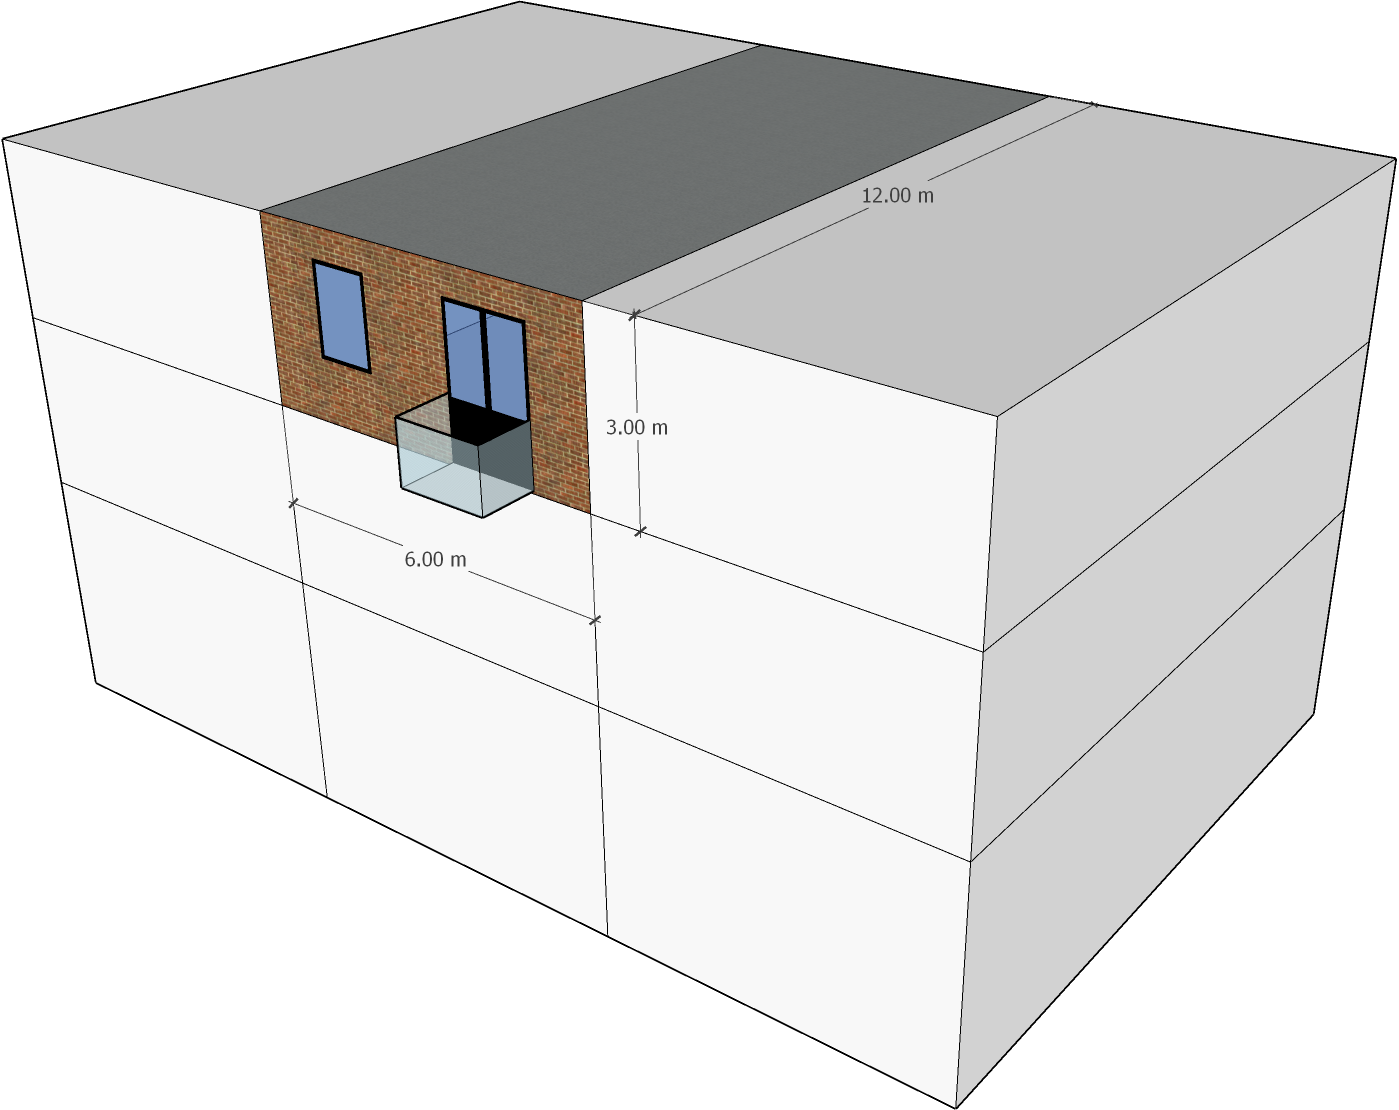
\includegraphics[height=9\baselineskip]{pictures/plex-unit}};

\end{slide}



% Données incomplètes
\begin{slide}[Les manufacturiers ne donnent pas suffisamment\\
			  d'informations sur les performances%
			  \only<5->{, ni sur le contrôle}]

\only<1>{
\begin{axis}[plot options, clip=false,
			 at={(p5cl cs:2,2)},
			 width=\bigcol+2\baselineskip, height=12\baselineskip,
			 xtick={-26.1, 15},
			 xticklabels={\num{-26.1}\phantom{$-$},
			 			  \phantom{\,\si{\celsius}}\SI{15}{\celsius}},
			 ytick={1.42, 4.75},]
\foreach \i in {1, ..., 4}{
	\addplot[mark=*, mark size=1pt, semithick] table[x=Toa, y=COP_at_T\i]
		{data/manu-data-heating.tsv};}
\foreach \i/\COP in {1/4.75, 2/4.524, 3/4.339, 4/3.961}{%
	\edef\temp{\noexpand\node (T\i) at (axis cs:15,\COP) {};}
	\temp}
\end{axis}
\node[anchor=mid west, font=\footnotesize] at (p5cl cs:1,14) {COP};
\node[anchor=base east, font=\footnotesize] (Toa)
	at (t5cr cs:4,0) {\To};
\foreach \i/\Ti in {1/15.6, 2/18.3, 3/21.1, 4/23.8}{
	\node[font=\footnotesize, gray, anchor=east] (Tr\i)
		at (T\i -| Toa.east) {\SI{\Ti}{\celsius}};
	\draw[gray] (T\i)++(4.5pt,0) -- ($(Tr\i.west)-(4pt,0)$);}
\node[anchor=west, yshift=-2\baselineskip, font=\footnotesize]
	at (Tr4.west) {\Tr};
}

\def\displayat{2}
\foreach \row/\rowlabel in {0/3, 1/2, 2/1}{
	\foreach \col/\collabel in {2/1, 3/2, 4/3}{
		\colorlet{background}{gray!10}
		\ifnum \row=2
			\ifnum \col=2
				\temporal<3>{
					\colorlet{background}{gray!10}}{
					\colorlet{background}{gray!10}}{
					\colorlet{background}{col!20}}
			\fi
		\fi
		\ifnum \col=2
			\renewcommand\displayat{2}
		\else
			\renewcommand\displayat{3}
		\fi
		\begin{axis}[visible on=<\displayat-4>,
					 enlargelimits=false, scale only axis,
					 hide axis,
					 at={($(p5cl cs:\col,0)+(0,56*\row*\quantum/3)$)},
					 width=\colv, height=11\baselineskip/3,
					 axis background/.style={fill=background}]
		
		\foreach \i in {1, ..., 4}{
			\addplot[mark=*, mark size=.5pt] table[x=Toa, y=COP_at_T\i]
				{data/manu-data-heating.tsv};}
			
		\end{axis}
		\ifnum \row=0
			\node[xshift=.5\colv, anchor=base, visible on=<3-4>]
				at (p5cl cs:\col,14){\ma[\collabel]};
		\fi
	}
	\pgfmathparse{2+\row}\let\labelypos\pgfmathresult
	\node[anchor=east, visible on=<2-4>] (row\row)
		at ($(p5cr cs:1,0)+(0,{(22+56*\row)*\quantum/3})$)
		{\fc[\rowlabel]};
}

\node[anchor=base] (pct) at ($(t5cl cs:0,6)!0.5!(row1.base west)$)
	{$ {\uncover<4>{{\color{col}1}\above 0.4pt} \uncover<3-4>{3 \times 3}}
	   \uncover<4>{\approx \SI{11}{\percent}} $};

\uncover<3-4>{
	\node[align=left, font=\footnotesize] (required)
		at (pct.202 |- row0) {paires $ (f, \dot m) $\\nécessaires};
	\draw (pct.202)++(0,-4pt) -- ($(required.north)+(0,4pt)$);}
\uncover<4>{
	\node[align=left, font=\footnotesize] (provided)
		at (pct.158 |- row2) {paire $ (f, \dot m) $\\fournie};
	\draw[col] (pct.158)++(0,4pt) -- ($(provided.south)-(0,4pt)$);}


\node[anchor=base west, align=left, visible on=<5>] at (t5cr cs:1,2){
	\begin{minipage}[b]{3\colvsep}\raggedright
	\hskip-.8pt Beaucoup de ``cas spéciaux'' sont détaillés,\\~\\
	\begin{listed}
		\item les limites d'opération\\
			  {\footnotesize\color{gray} fréquences minimale et maximale,
			  							 \ldots}
		\item le contrôle des ventilateurs\\
			  {\footnotesize\color{gray} vitesse en fonction
			  							 de la température}
		\item le contrôle du mode d'opération\\
			  {\footnotesize\color{gray} chauffage ou climatisation,
			  							 selon la consigne}
	\end{listed}
	\vskip\baselineskip \hskip-.8pt mais pas le contrôle normal
									de la fréquence 
	\end{minipage}};

\end{slide}



\begin{slide}[Les stratégies de contrôle et les performances\\ 
			  sont évaluées expérimentalement]

\node[anchor=north west] at (p5cl cs:.25,15)	{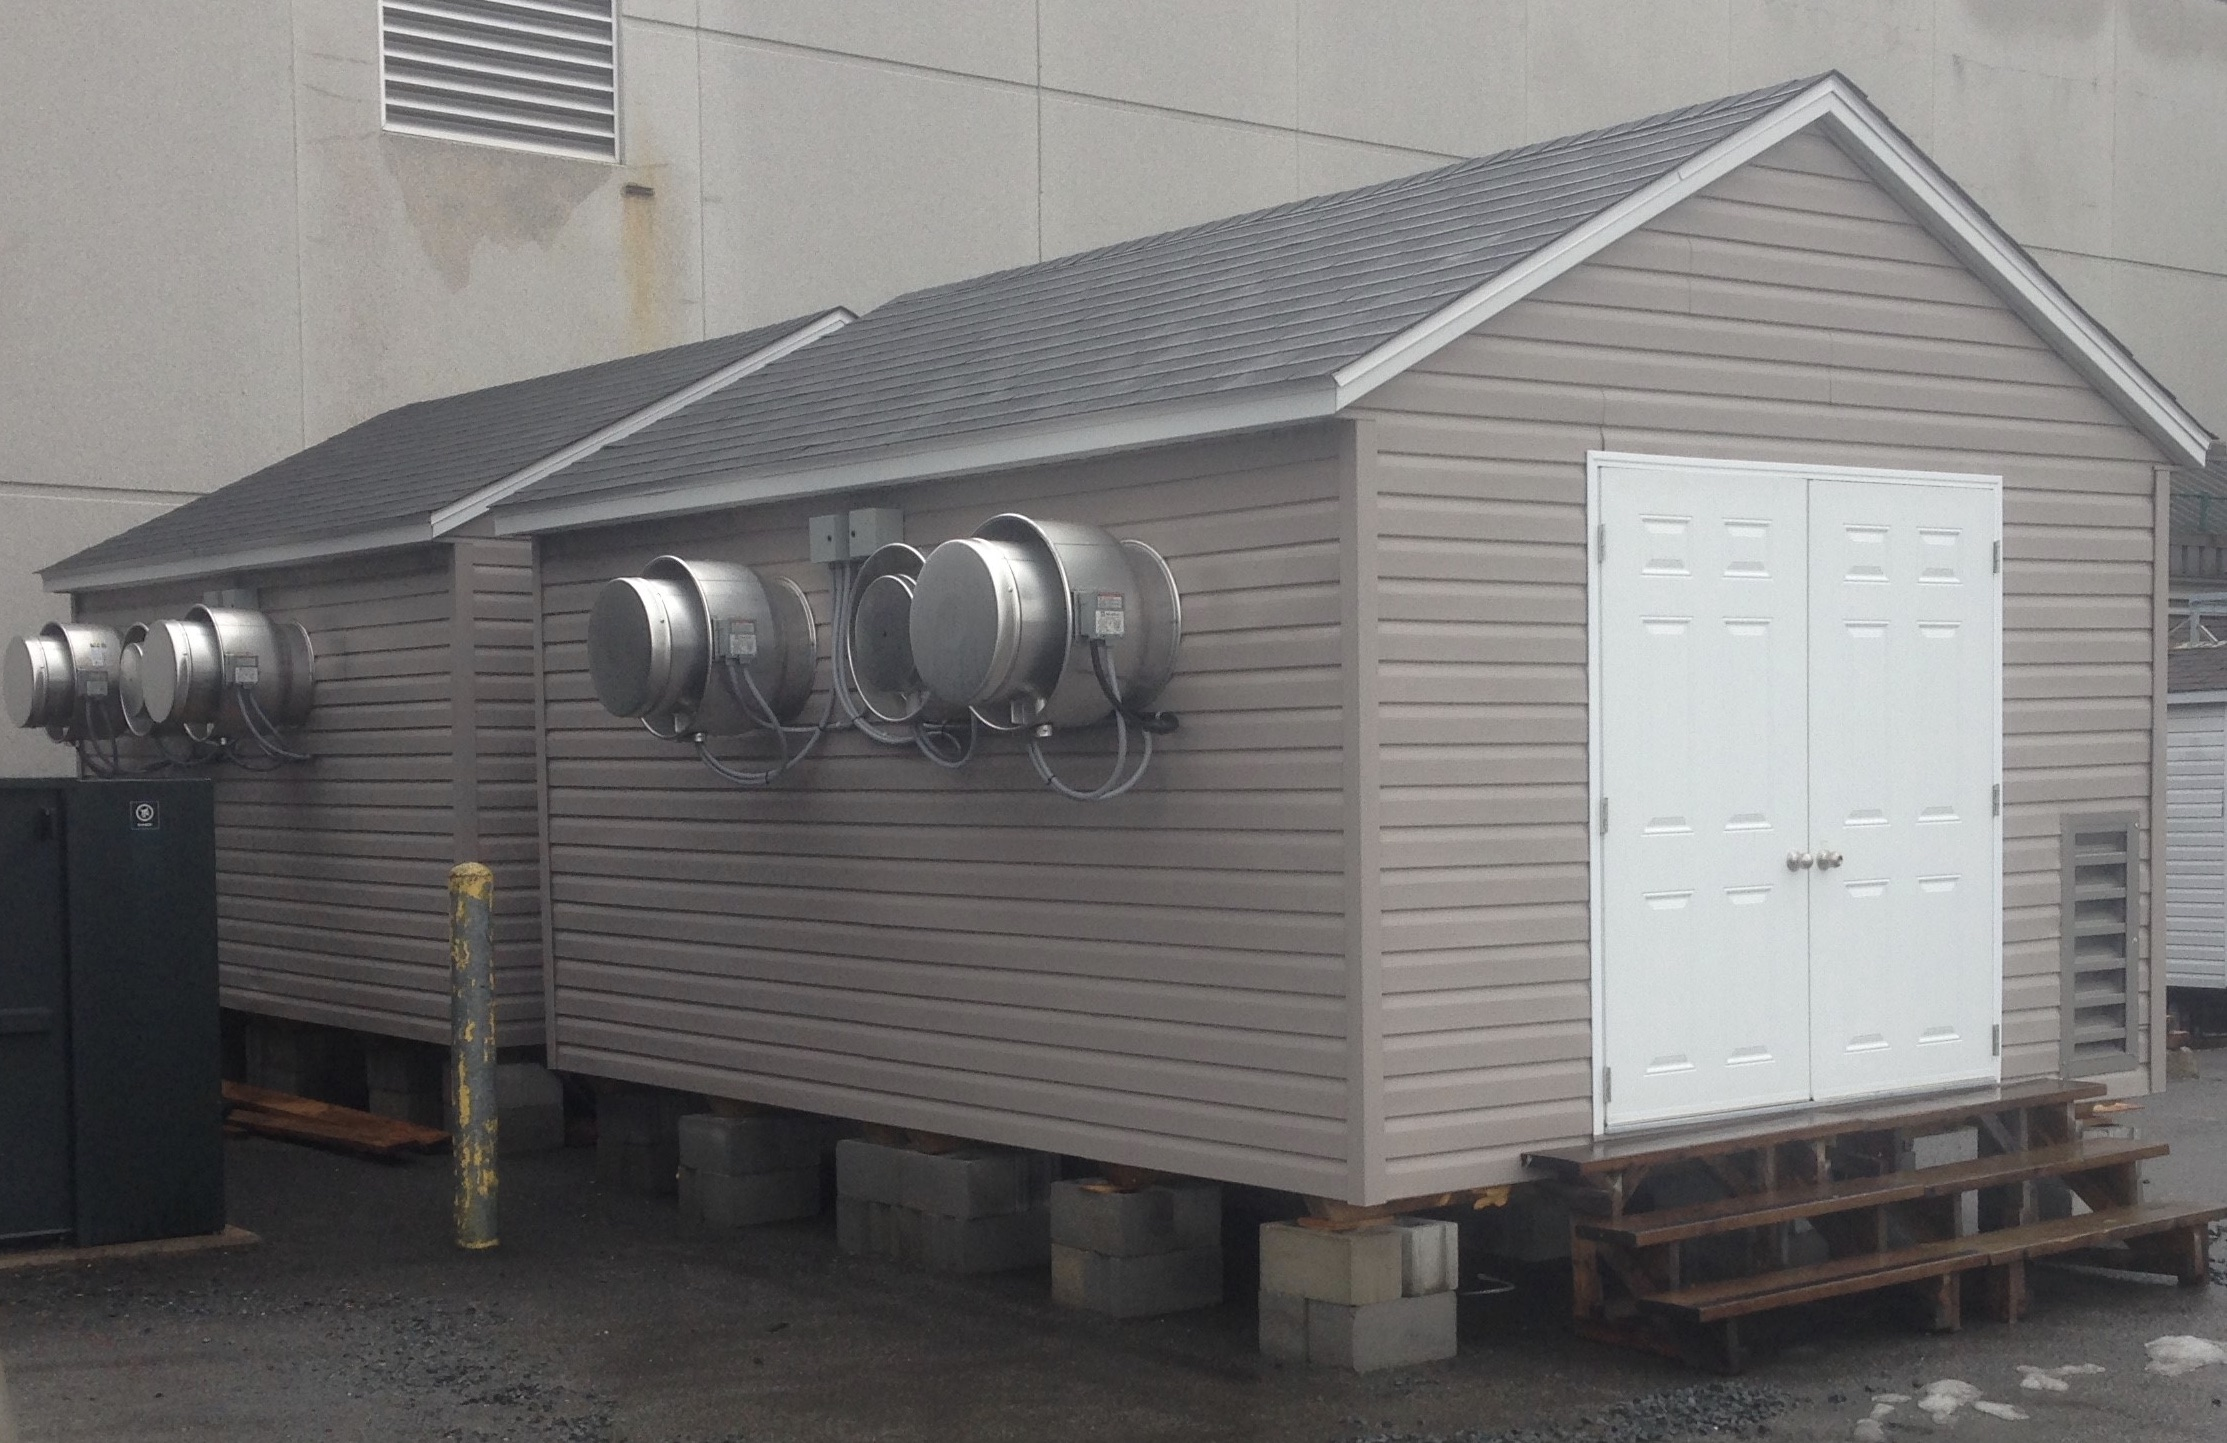
\includegraphics[width=2\colvsep]{pictures/sheds}};
\node[anchor=south west] at (p5cl cs:.25,0)
	{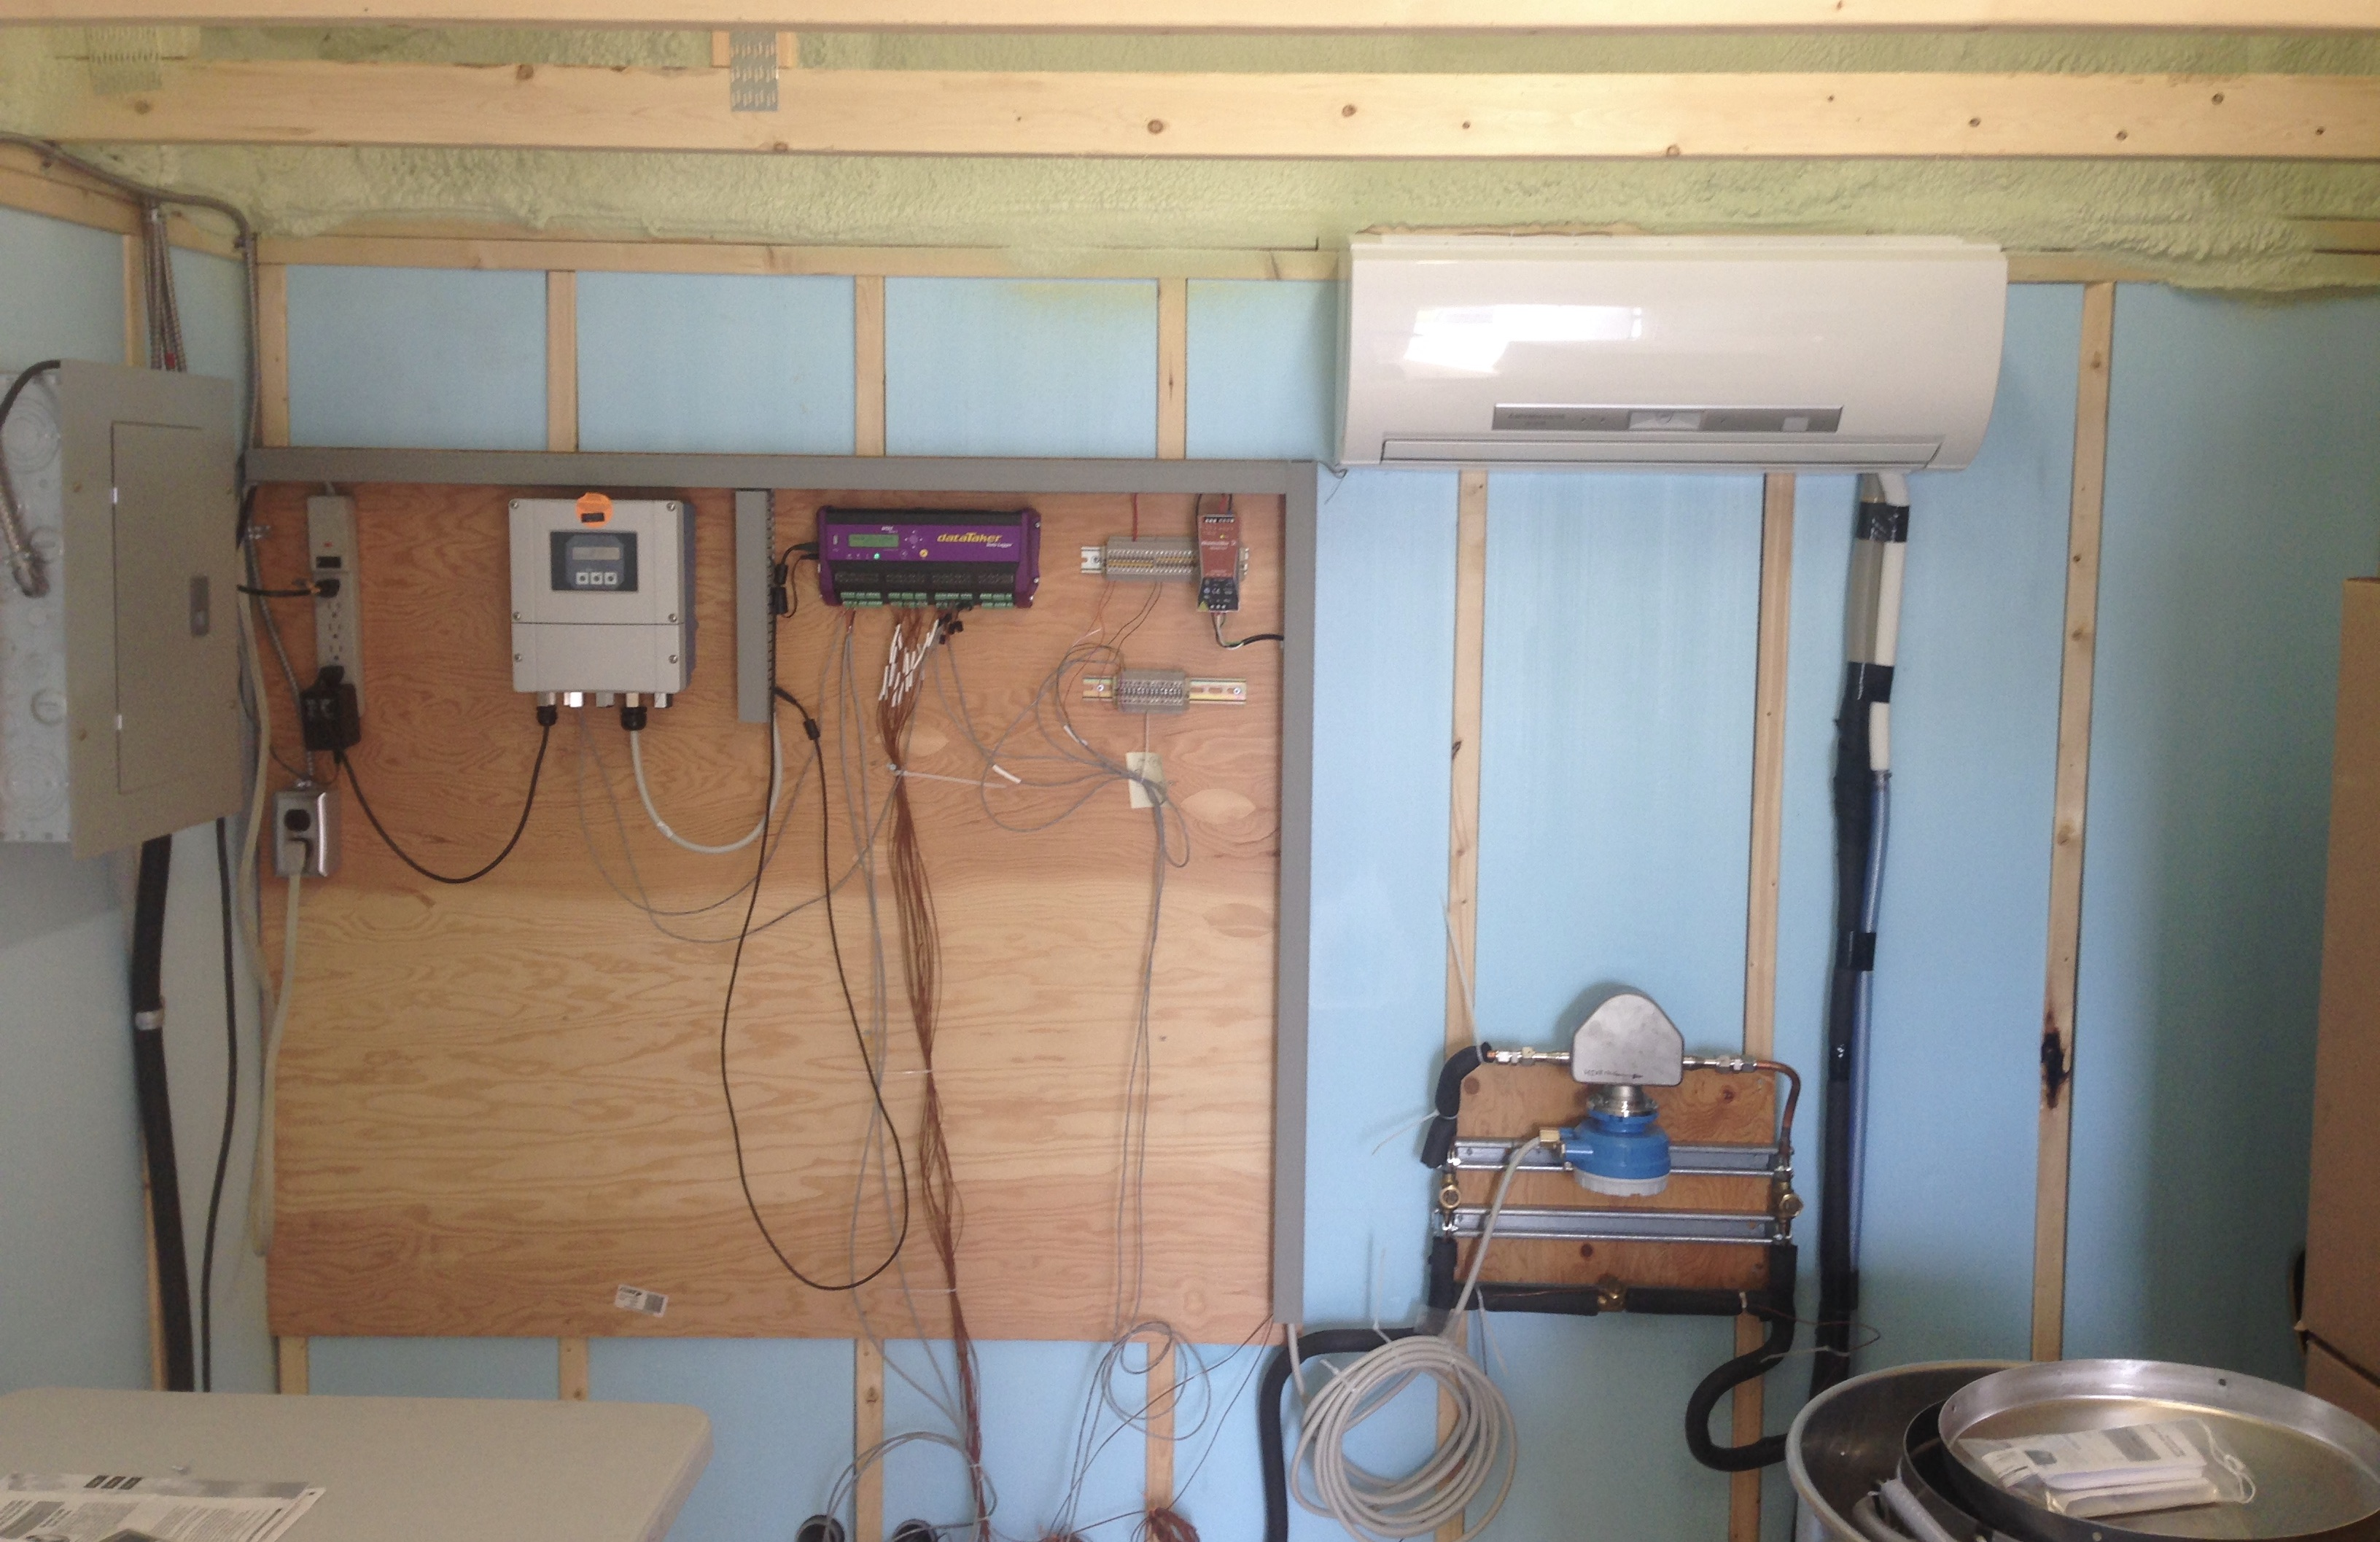
\includegraphics[width=2\colvsep]{pictures/indoor-unit}};
\node[anchor=south east] at (p5cr cs:3.75,0)
	{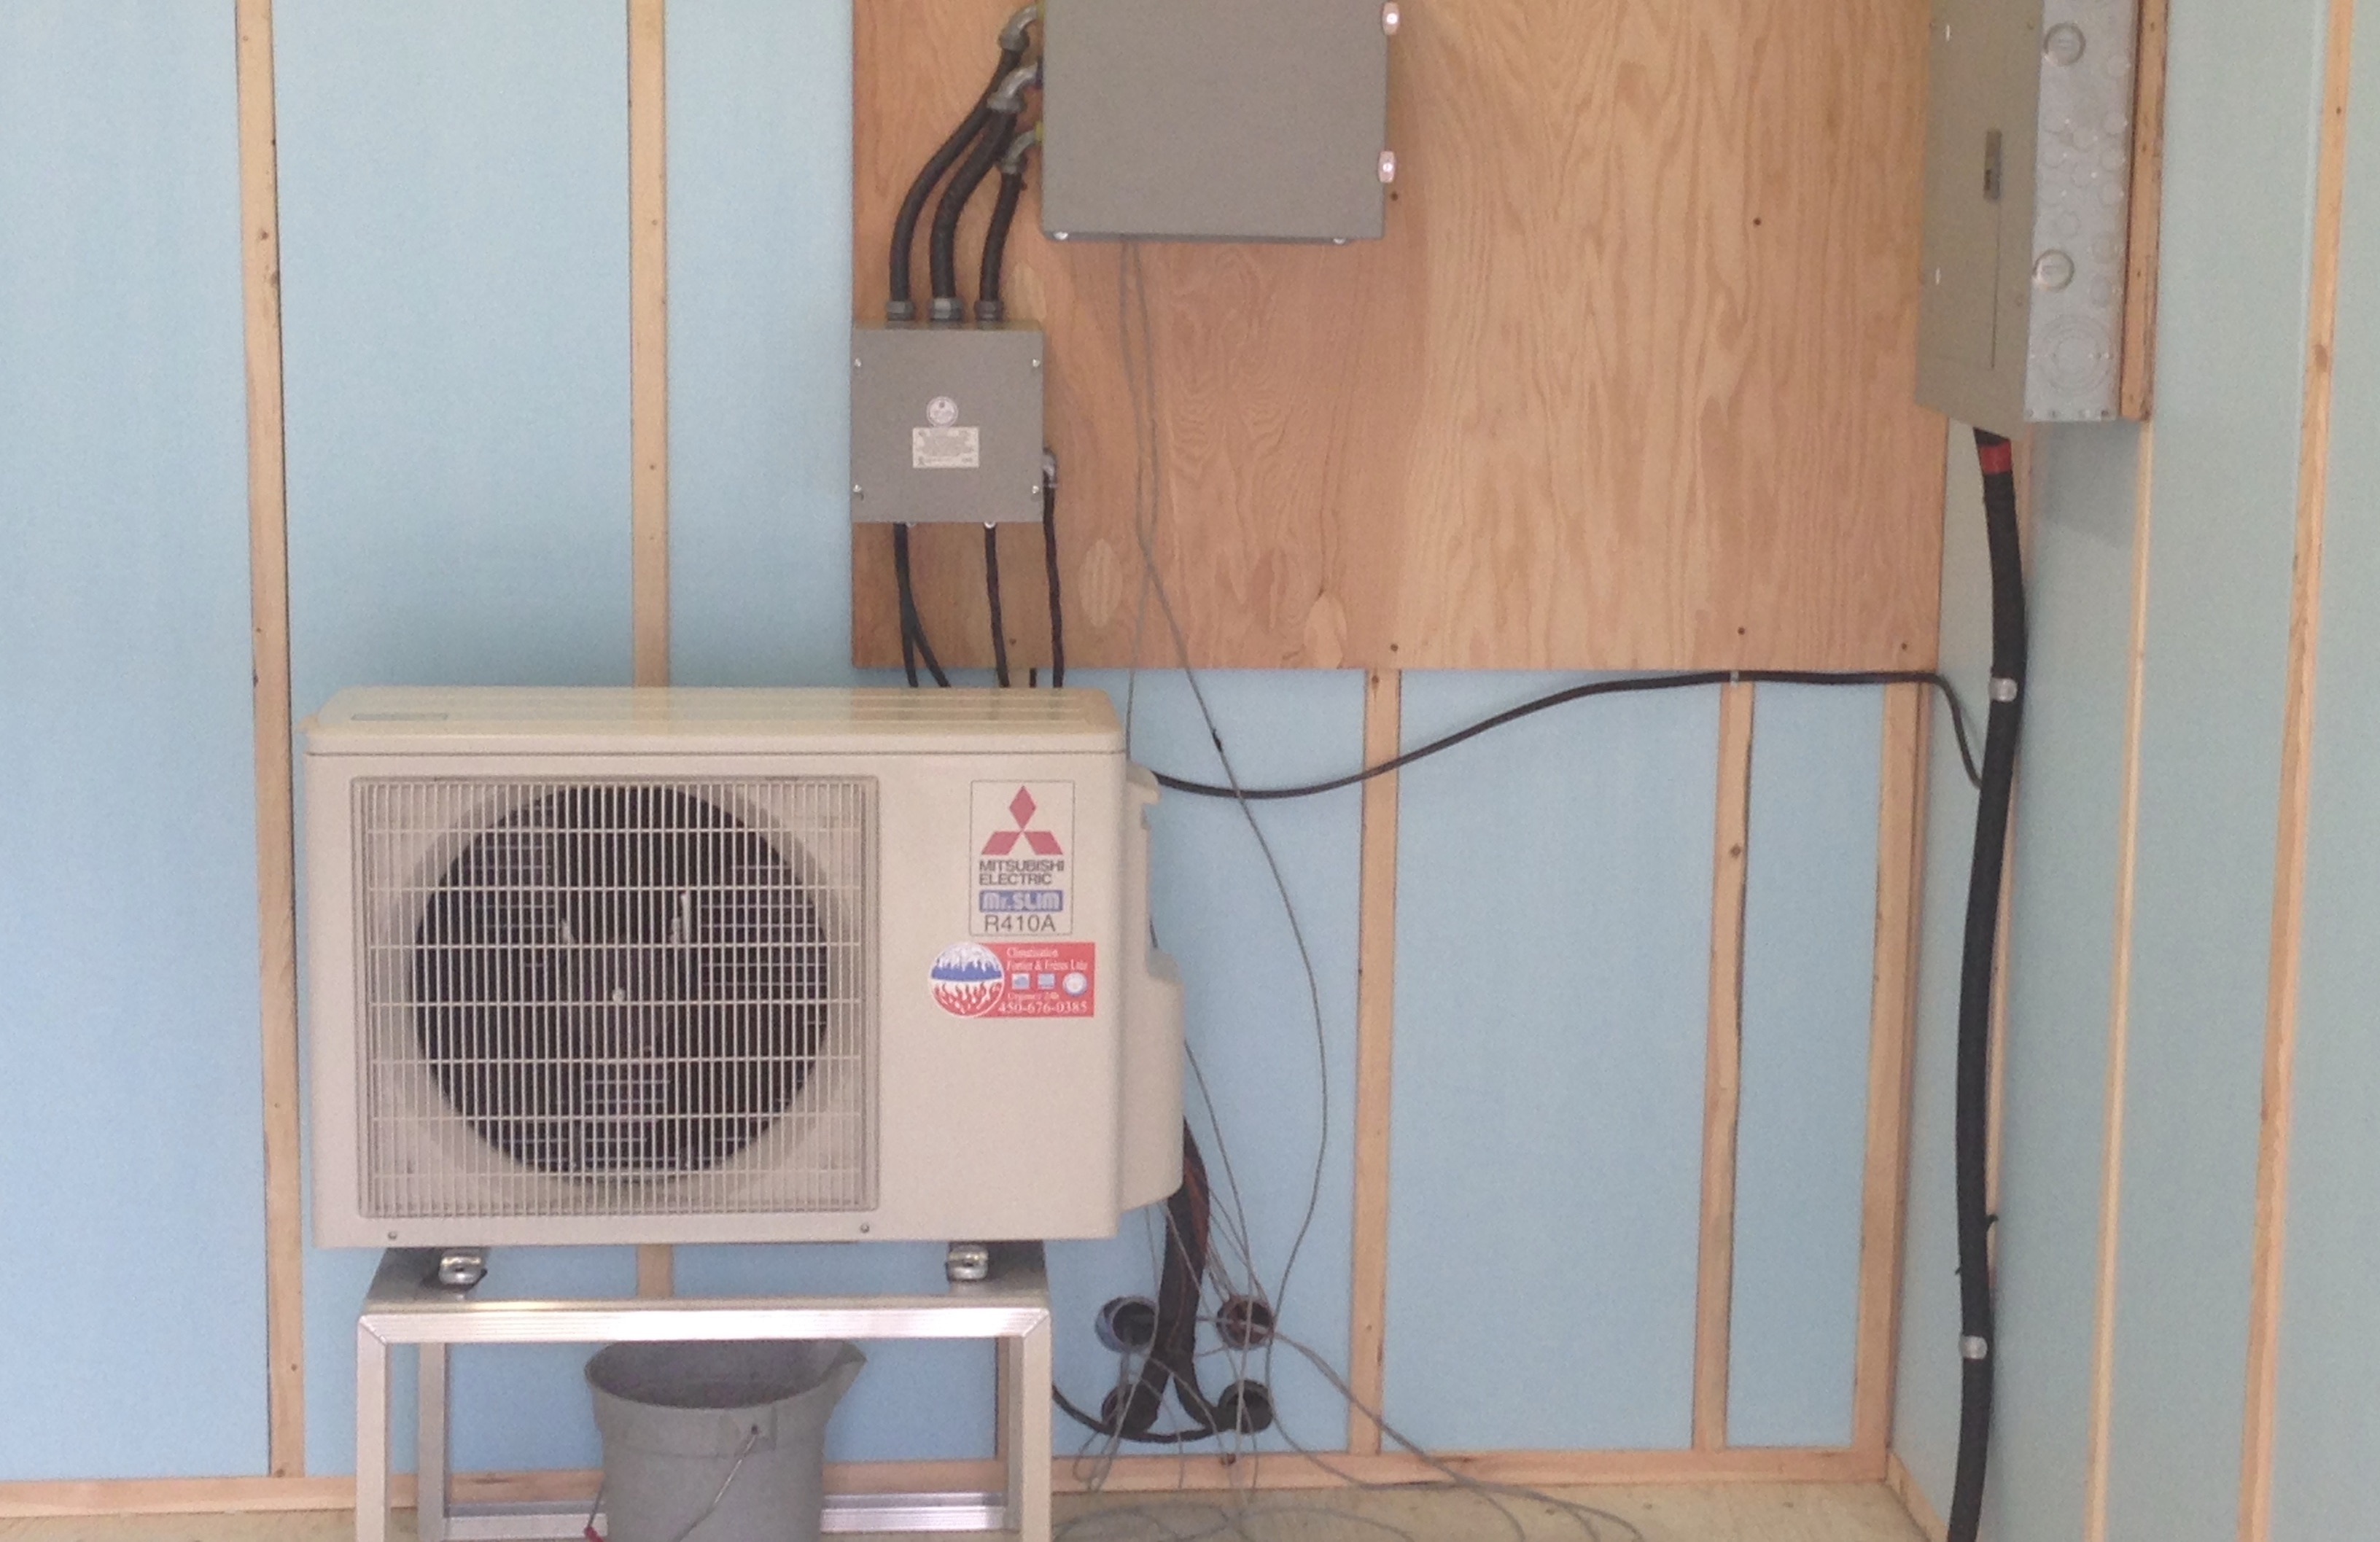
\includegraphics[width=2\colvsep]{pictures/outdoor-unit}};

\node[anchor=base east] at (t5cr cs:3.75,8){
	\begin{minipage}[b]{2\colvsep}
		Pour obtenir les performances dans les conditions désirées,
		\begin{listed}
		\setlength\itemsep{0pt}
			\item la charge
			\item la température extérieure
			\item le débit d'air
		\end{listed}
		sont imposés en contrôlant la quantité d'air entrant
	\end{minipage}};

\end{slide}



\begin{slide}[Le modèle parvient à prévoir les performances\\
			  \only<2>{et à reproduire les principaux comportements}]

\only<1>{
\begin{groupplot}[group style={group size=1 by 2,},
				  width=\bigcol+\colvsep,
				  xmin=0, xmax=3,
				  clip=false,
				  plot options,]
\nextgroupplot[
	height=3\baselineskip,
	axis x line=none,
	ymin=3.5, ymax=3.8,
	ytick={3.5, 3.8},
	yticklabels={3.5,\SI{3.8}{\kilo\watt}},
	at={(p5cr cs:1,10)},
	anchor=south west,
	]
\addplot[thick, gray] table[x=TIME, y=Qc-exp] {data/cooling-io.tsv};
\addplot[thick,  col] table[x=TIME, y=Qc-sim] {data/cooling-io.tsv};
\draw[latex-] (axis cs:1.7, 3.76) |- ++(3\quanta, 4\quanta)
	node[right, inner sep=3pt] {\footnotesize \SI{6.5}{\percent} error};
\draw[latex-] (axis cs:1.7, 3.5148) |- ++(0mm, -4\quanta);

\nextgroupplot[
	height=3\baselineskip,
	xtick={0, 3},
	xticklabels={0, \phantom{h\,}\SI{3}{\hour}},
	ymin=0.84, ymax=0.94,
	ytick={0.84, 0.94},
	yticklabels={840,\SI{940}{\watt}},
	at={(p5cr cs:1,3)},
	anchor=south west,
	]
\addplot[thick, gray] table[x=TIME, y=Pel-exp] {data/cooling-io.tsv};
\addplot[thick, col] table[x=TIME, y=Pel-sim] {data/cooling-io.tsv};
\draw[latex-] (axis cs:0.5833, 0.91648) |- ++(3\quanta, 4\quanta)
	node[right, inner sep=3pt] {\footnotesize \SI{8}{\percent} error};
\draw[latex-] (axis cs:0.5833, 0.84669) |- ++(0mm, -4\quanta);

\end{groupplot}

\node[anchor=mid west] at (p5cr cs:0,13) {\footnotesize\Qc};
\node[anchor=mid west] at (p5cr cs:0,6) {\footnotesize\Pel};
\node[gray, anchor=base west] at (t5cr cs:1.4,13.5)
	{\scriptsize measurements};
\node[col, anchor=base west] at (t5cr cs:1.4,9) {\scriptsize simulation};
}


\only<2>{
\begin{groupplot}[group style={group size=1 by 3,},
				  width=\bigcol+\colvsep,
				  xmin=0, xmax=4,
				  clip=false,
				  plot options,]
\nextgroupplot[
	height=3\baselineskip,
	axis x line=none,
	ymin=0, ymax=57,
	ytick={0, 57},
	yticklabels={0, \SI{57}{\hertz}},
	at={(p5cr cs:1,11)},
	anchor=south west,
	]
\addplot[thick, gray] table[x=TIME, y=f-exp] {data/cooling-sim.tsv};
\addplot[thick, col] table[x=TIME, y=f-sim] {data/cooling-sim.tsv};


\nextgroupplot[
	height=2\baselineskip,
	axis x line=none,
	ymin=14, ymax=24,
	ytick={14, 24},
	yticklabels={14, \SI{24}{\celsius}},
	at={(p5cr cs:1,7)},
	anchor=south west,
	]
\addplot[thick, gray] table[x=TIME, y=Ts-exp] {data/cooling-sim.tsv};
\addplot[thick, col] table[x=TIME, y=Ts-sim] {data/cooling-sim.tsv};
\draw[latex-] (axis cs:2.6, 17.373) |- ++(3\quanta, 4\quanta)
	node[right, inner sep=3pt] {\footnotesize\SI{3.7}{\celsius}};
\draw[latex-] (axis cs:2.6, 13.689) -- ++(0mm,-4\quanta);


\nextgroupplot[
	height=3\baselineskip,
	xtick={0, 4},
	xticklabels={0, \phantom{h\,}\SI{4}{\hour}},
	ymin=23, ymax=44,
	ytick={23, 44},
	yticklabels={23, \SI{44}{\celsius}},
	at={(p5cr cs:1,2)},
	anchor=south west,
	]
\addplot[thick] table[x=TIME, y=Toa] {data/cooling-sim.tsv}
	node[pos=0.7, fill=white, font=\footnotesize, inner sep=3pt] {\To};
\addplot[thick, gray] table[x=TIME, y=Tr-exp] {data/cooling-sim.tsv};
\addplot[thick, col] table[x=TIME, y=Tr-sim] {data/cooling-sim.tsv};

\end{groupplot}

\node[anchor=mid west] at (p5cr cs:0,14) {\footnotesize\fc};
\node[anchor=mid west] at (p5cr cs:0,9) {\footnotesize\Ts};
\node[anchor=mid west] at (p5cr cs:0,5) {\footnotesize\Tr};
}


\end{slide}

\map

\section{Banc d'essai}
\map[1]
\begin{slide}[Les environnements intérieur et extérieur\\
			  sont chacun contrôlés dans un cabanon séparé]

\begin{scope}[shift={(p5cl cs:0,3)}, x=.25\bigcol, y=\baselineskip]

\node[anchor=base, gray] at (2, 10.25) {zone intérieure};
\fill[gray!20] (0,0) -| (4,6) -- (2,9)
			-- (0,6) |- (.2,5) |- (0,3.25) -- cycle;

% indoor unit
\node[minimum width=1cm, minimum height=3mm, rectangle, draw, thick,
	  rounded corners=.25\quantum] (IU) at (2.5,4.5) {};
\fill[gray!60!black] (IU.202) |- (IU.338 |- IU.west) |- cycle;
\path (.1,4.125) pic [rotate=90, thick] {fan=.4} node[dot, scale=1] {};

% points
\draw[latex-, col!50, thick] (IU.north) -- ++(0,1)
	node[dot, anchor=south, black, label={[black]above left:$r$}] (r) {};
\draw[-latex, col, thick] (IU.south) ++(0,.2) -- ++(0,-1)
	node[dot, anchor=north, black, label={[black]below left:$s$}] {};

% auxiliary heater
\draw[semithick] (0,.5) -- ++(.2,0)
	++(0,.16) rectangle ++(.6,-.33)++(0,.16)
	-| node[right, xshift=3pt] {\Lightning} ++(.2,-.5)
	foreach \x in {.35,.5,.65}{(\x,.66) -- (\x,.34)};

\end{scope}



\begin{scope}[shift={(p5cl cs:3,3)}, x=.25\bigcol, y=\baselineskip]

\node[anchor=base, gray] at (2, 10.25) {zone extérieure};
\fill[gray!20] (0,0) -| (4,3.25) -| (3.8,5) -| (4,6)
			-- (2,9) -- (0,6) -- cycle;
\path (3.9,4.125) pic [rotate=90, thick] {fan=.4} node[dot, scale=1] {};

% outdoor unit
\node[minimum width=1cm, minimum height=6mm, rectangle, draw, thick,
	  rounded corners=.25\quantum] (OU) at (1.5,2.3) {};
\node[circle, draw, minimum size=4\quanta] (grid) at ($(OU)-(.15,0)$) {};
\draw[ultra thin] foreach \angle in {-54, -36, ..., 54}{
	(grid.\angle) -- (grid.{180-\angle})
	(grid.{90+\angle}) -- (grid.{-90-\angle})};
\node[circle, fill=gray!60!black, scale=4]
	at ($(grid.east)!0.5!(OU.east)$) {};

% points
\coordinate (C1) at (2,0);
\node[dot, label={[black, yshift=3pt]above:$o$}] at (IU -| C1) {};

% auxiliary heater
\draw[semithick] (4,.5) -- ++(-.2,0)
	++(0,.16) rectangle ++(-.6,-.33)++(0,.16)
	-| node[left, xshift=-3pt] {\Lightning} ++(-.2,-.5)
	foreach \x in {.35,.5,.65}{(4-\x,.66) -- (4-\x,.34)};

\end{scope}


% refrigerant lines
\only<1>{
\draw[col, midarrow=0.5-latex, semithick] (OU.west)++(0,.05)
	-| ($(IU.east)+(.55,.05)$) -- ($(IU.east)+(0,.05)$);
\draw[gray, midarrow=0.65-latex, semithick] (IU.east)++(0,-.05)
	-- ++(.45,0) |- ($(OU.west)-(0,.05)$);
}
\only<2>{
\draw[gray, midarrow=0.65-latex, semithick] (IU.east)++(0,.05) -- ++(.55,0)
	|- ($(OU.west)+(0,.05)$);
\draw[col, midarrow=0.5-latex, semithick] (OU.west)++(0,-.05)
	-| ($(IU.east)+(.45,-.05)$) -- ($(IU.east)-(0,.05)$);
}

% heat flux
\only<1>{
\node[becomes, rotate=90, anchor=south,
	  label={[left, label distance=\quantum]:\Qh}]
	at ($(IU.west)-(2\quanta,0)$) {};
\node[becomes, rotate=90, anchor=north,
	  label={[right, xshift=3.5\quanta]:$\skew{5}\dot Q_\text{abs}$}]
	at ($(OU.east)+(2\quanta,0)$) {};
}
\only<2>{
\node[becomes, rotate=-90, anchor=north,
	  label={[left, xshift=-3.5\quanta]:\Qc}]
	at ($(IU.west)-(2\quanta,0)$) {};
\node[becomes, rotate=-90, anchor=south,
	  label={[right, xshift=\quantum]:$\skew{5}\dot Q_\text{rej}$}]
	at ($(OU.east)+(2\quanta,0)$) {};
}

\end{slide}




\begin{slide}[Le débit d'air de l'unité intérieure\\
			  est mesuré avec un \emph{duct blaster}]


\begin{scope}[shift={(p5cl cs:0.3,6)}]

% air flux
\draw[line width=1mm, -{Triangle[scale=0.7]}, col!50] (.2,3.4)
	node[above, yshift=1mm, black] {$r$} to[out=270, in=110] (.35,2.4);
\draw[line width=1mm, -{Triangle[scale=0.7]}, col] (.4,2.25)
	to[out=320, in=180] (1.4,1.95) node[right, black, xshift=1mm] {$s$};

% indoor unit
\filldraw[gray!50, very thick] (0,3) rectangle (-.2,2);
\draw[dotted] (0,3) -- (0.5,3);
\draw[very thick, line cap=rect] (.5,3) -- (1,3) node (IU) {}
									 to[out=270, in=60] (.9,2.3)
								 (0,3) |- (0.5,2) -- ++(340:.2)
								 (.75,2.15) -- ++(340:.2);

% plenum
\draw[semithick] (1,2.8) -- (2,2.8) -- (3,2.5)
	  (.25,2) |- (2,1) -- (3,1.3);

% join
\filldraw[semithick] (3,2.5) rectangle (3.2,1.3);

% duct
\draw[semithick, gray] (3.2,2.5) arc (90:20:2.2) -- ++(290:1.5)
	arc(200:270:1) node (N0) {} -- ++(1.2,0) node (N1) {};
\draw[semithick, gray] (3.2,1.3) arc (90:20:1) -- coordinate (C1)
	++(290:1.5) arc (200:270:2.2) -- ++(1.2,0) node (N2) {};
\draw[gray] foreach \theta in {20, 30, ..., 90}{
				(3.2,.3)++(\theta:1) -- ++(\theta:1.2)}
            foreach \x in {0.3, 0.6, ..., 1.5}{
            		(3.2,.3)++(20:1)++(290:\x) -- ++(20:1.2)}
            foreach \theta in {200, 210, ..., 270}{
            		(N0)++(0,1)++(\theta:1)    -- ++(\theta:1.2)}
            foreach \x in {0.3, 0.6, 0.9}{
            		(N0)++(\x,0) -- ++(0,-1.2)};

% join
\filldraw[thick] (N1)++(.2,0) rectangle (N2);

% fan casing
\draw[thick] (N1)++(.2,0) arc (270:360:.1) |- node (D1) {} ++(.7,.2)
		-- ++(0,-.3) node (P1) {}
			 (N2)++(.2,0) arc (90:0:.1)    |- ++(.7,-.2) node (D2) {}
		-- ++(0,.3) node (P2) {};

\draw foreach \y in {-.45,-.3,...,.45}{
	($(P1)!0.5!(P2)-(.05,\y)$) -- ++(.1,0) };

% fan
\path ($(D1)!0.5!(D2)$) pic [rotate=90, thick] {fan2=2} node[dot] (F) {};

% outlet air flux
\draw[line width=1mm, -{Triangle[scale=0.7]}, col] ($(P1)!0.5!(P2)+(.2,0)$) -- ++(.7,0);

% labels
\draw[gray, semithick] (IU)++(45:3pt) -- ++(45:.7) -- ++(.7,0)
	node[anchor=mid west, inner sep=3pt] {unité intérieure};

\draw[gray, semithick] (D1.north -| F)++(0,3pt) -- ++(0,1)
	node[above, inner sep=3pt] {duct blaster};

\draw[gray, semithick] (C1)++(200:3pt) -- ++(200:.7) -- ++(-.7,0)
	node[anchor=mid east, inner sep=3pt] {conduit flexible};

\end{scope}

\end{slide}





\setlength{\templen}{7\baselineskip}

\begin{slide}[Les capacités totales sont plus facilement calculées\\
			  avec les propriétés du réfrigérant]


\begin{scope}[shift={(p5cl cs:0,4)}, visible on=<{1,4-5}>]

% four-way valve 
\coordinate [circle, draw, thick, minimum size=7mm]
	(4wValve) at (\templen, 0.5\templen) {};

% compressor
\coordinate [compressor, draw, thick, minimum size=7mm,
			 right=\bigcol-\templen of 4wValve.center, anchor=center]
	(comp);

% indoor unit HX
\draw[thick, HX] (0.5\templen-5mm,\templen) node (iuOut) {} --
	node [yshift=2\baselineskip, gray] {\scriptsize unité intérieure}
	++(1,0) node (iuIn) {};

% expansion valve
\coordinate [expValve] (v) at (0,0.5\templen) {};

% outdoor unit HX
\draw [HX, thick] (0.5\templen-5mm,0) node(ouIn){} --
	node [yshift=-2\baselineskip, gray] {\scriptsize unité extérieure}
	++(1,0) node (ouOut) {};

% refrigerant lines, heating
\begin{scope}[visible on=<{1,4}>]

\draw[thick, midarrow=.75-latex, col!50]
	(ouOut.center) -| coordinate (6h) (4wValve.225);
\coordinate (C0) at ($(4wValve.225)!0.5!(ouOut)$);
\draw[thick, col!50, line cap=rect]
	(4wValve.225)++(0,-.1) -- (4wValve.225)
	arc (135:45:3.5mm) -- (C0 -| 4wValve.315) coordinate (C1);
\draw[thick, midarrow=.4-latex, col!50]
	(C1) -| coordinate (1) (comp.south);
\coordinate (C2) at ($(4wValve.45)!0.5!(iuIn)$);
\draw[thick, midarrow=.5-latex, col]
	(comp.north) |- coordinate (2) (4wValve.135 |- C2) -- (4wValve.135);
\draw[thick, col] (4wValve.135)++(0,.1) -- ++(0,-.1) arc (225:315:3.5mm)
	coordinate (C3) -- ($(2 -| C3)-(0,.05)$) ++(0,.1) coordinate (C4);
\draw[thick, midarrow=.75-latex, col]
	(C4) |- coordinate (3) (iuIn.center);
\draw[thick, midarrow=.8-latex, gray]
	(iuOut.center) -| coordinate (4) (v.north);
\draw[thick, midarrow=.85-latex, gray!50]
	(v.south) |- coordinate (5h) (ouIn.center);

\end{scope}

% refrigerant lines, cooling
\begin{scope}[visible on=<5>]

\coordinate (C0) at ($(4wValve.225)!0.5!(ouOut)$);
\coordinate (C2) at ($(4wValve.45)!0.5!(iuIn)$);
\draw[thick, midarrow=.5-latex, col]
	(comp.north) |- coordinate (2) (4wValve.135 |- C2) -- (4wValve.135);
\draw[thick, col, midarrow=.53-latex] (4wValve.135)++(0,.1) -- ++(0,-.1)
	arc (45:-45:3.5mm) |- coordinate (6) (ouOut.center);
\draw[thick, midarrow=.8-latex, gray]
	(ouIn.center) -| coordinate (5) (v.south);
\draw[thick, midarrow=.85-latex, gray!50]
	(v.north) |- coordinate (4c) (iuOut.center);
\draw[thick, midarrow=.3-latex, col!50] (iuIn.center) -| coordinate (3c)
	($(C2 -| 4wValve.45)+(0,.05)$) ++(0,-.1) -- (4wValve.45);
\draw[thick, col!50, line cap=rect] (4wValve.45)++(0,.1) -- ++(0,-.1)
	arc (135:225:3.5mm) -- (C0 -| 4wValve.315) coordinate (C1);
\draw[thick, col!50, midarrow=.4-latex] (C1) -| coordinate (1) (comp.south);

\end{scope}

% re-draw valve to avoid overlap
\node[expValve, thick] at (v) {};

\tikzset{inner sep=3pt, font=\scriptsize}
% refrigerant states
\foreach \sensor/\lab/\pos in {1/1/below right, 2/2/above right,
							   3/3/above right, 4/4/above left,
							   5h/5/below left, 6h/6/below right}{
	\node[dot, label=\pos:\lab] at (\sensor) {};}

\end{scope}


\node[anchor=base west, visible on=<{2-3,6}>,
	  background text=gray, text on=<{3,6}>] at (t5cl cs:0,9)
	{$ \Pcp = \mr(h_2 - h_1) $};
\node[anchor=base west, visible on=<{3,6}>,
	  background text=gray, text on=<6>] at (t5cl cs:0,7)
	{$ \Qh = \mr(h_3 - h_4) + \Pfi $};
\node[anchor=base west, visible on=<6>] at (t5cl cs:0,5)
	{$ \Qc = \mr(h_3 - h_4) - \Pfi $};


\begin{scope}[shift={(p5cl cs:3,5)}, x=\bigcol/5,
			  y=4\baselineskip/1.7183, xshift=.1\bigcol]

\tikzset{inner sep=3pt, font=\scriptsize}

\coordinate (LVEbottom) at (2.4,-\baselineskip);
\fill[gray!20] (-.5,-\baselineskip) to [out=65, in=220] (1,2.65)
	to [out=40,in=180] (1.6,2.8) coordinate (SC)
	to [out=0, in=80] coordinate[pos=0.3] (LVE) (LVEbottom);
\only<1>{
	\node[gray, align=left, font=\scriptsize, anchor=base east]
		(LVElab) at (t5cr cs:4,12) {Équilibre\\liquide-vapeur};
	\draw[gray] (LVElab.base -| LVElab.230)++(0,-3pt) -- ++(0,-.4)
		coordinate (C1) -- ($(C1)!0.8!(LVE)$);}

\draw[midarrow=0.55-latex, hl=draw on <6>]
	(0,0) coordinate[dot, hl=fill on <6>] (evi) --
	(2.6,0) coordinate[dot, hl=fill on <6>] (evo);
\draw (evo) -- (3,0) coordinate (cpi);
\draw[midarrow=0.55-latex, hl=draw on <2>]
	(cpi) node[dot, hl=fill on <2>] {} --
	plot[domain=3:4.5] (\x, {exp(\x/1.5-2) - 1})
	coordinate[dot, hl=fill on <2>] (cpo);
\draw (cpo) -- ++(-.5,0) coordinate[dot, hl=fill on <3>] (cdi);
\draw[midarrow=0.5-latex, hl=draw on <3>] (cdi) -- (cpo -| evi)
	coordinate[dot, hl=fill on <3>] (cdo) {};
\draw[midarrow=0.55-latex] (cdo) -- (evi);

\node [below right, background text=col, text on=<2>] at (cpi) {1};
\node [above right, background text=col, text on=<2>] at (cpo) {2};
\node [above, background text=col, text on=<3>] at (cdi)
	{\temporal<4>{3}{3}{6}};
\node [above left, background text=col, text on=<3>] at (cdo)
	{\temporal<4>{4}{4}{5}};
\node [below left, background text=col, text on=<6>] at (evi)
	{\temporal<4>{5}{5}{4}};
\node[below, background text=col, text on=<6>] at (evo)
	{\temporal<4>{6}{6}{3}};


% axes
\draw[semithick, hlb=draw on <{3,6}>]
	(0,-8\quanta) node[below, hlb=text on <{3,6}>] {$ h_4 $}
	++(-.3pt,0) -- (2.6,-8\quanta) -- ++(.3pt,0);
\draw[semithick, hlb=draw on <3>] (2.6,-8\quanta)
	node[below, hlb=text on <6>] {$ h_{\temporal<4>{6}{6}{3}} $}
	++(.3pt,0) -- ($(3,-8\quanta)-(.3pt,0)$);
\draw[semithick, hlb=draw on <{2,3}>]
	(3,-8\quanta) node[below, hlb=text on <2>] {$ h_1 $}
	++(-.3pt,0) -- (4,-8\quanta) -- ++(.3pt,0);
\draw[semithick, hlb=draw on <2>] (4,-8\quanta)
	node[below, hlb=text on <3>] {$ h_{\temporal<4>{3}{3}{6}} $}
	++(.3pt,0) -- (4.5,-8\quanta) node[below, hlb=text on <2>] {$ h_2 $}
	-- ++(.3pt,0);
\draw[semithick, hlb=draw on <{3,6}>]
	(0,-8\quanta)++(0,.3pt) -- (0,-7\quanta);
\draw[semithick, hlb=draw on <6>]
	(2.6,-8\quanta)++(0,.3pt) -- (2.6,-7\quanta);
\draw[semithick, hlb=draw on <2>]
	(3,-8\quanta)++(0,.3pt) -- (3,-7\quanta);
\draw[semithick, hlb=draw on <3>]
	(4,-8\quanta)++(0,.3pt) -- (4,-7\quanta);
\draw[semithick, hlb=draw on <2>]
	(4.5,-8\quanta)++(0,.3pt) -- (4.5,-7\quanta);

\draw[gray, semithick]
	(-7\quanta,0) -| node[left] {$ p_{\temporal<4>{5}{5}{4}} = p_1 $}
	(-8\quanta,1.7183) node[left] {$ p_{\temporal<4>{4}{4}{5}} = p_2 $}
	-- +(\quantum,0);

\end{scope}

\end{slide}





\section{Stratégies de contrôle}
\map[2]
% MAP: PID
\begin{slide}[La fréquence est régulée avec un contrôleur PI]

\begin{scope}[shift={(p5cl cs:0,13)}, node distance=5mm,
			  font=\footnotesize, inner sep=3pt]

\node [anchor=west] (Tset) at (.1,0) {$ T_\text{set} $};
\node [right=of Tset, sum] (sum1) {$ \sum $};
\coordinate [dot, right=1cm of sum1] (N1);

\node [block, anchor=north west] (ki) at ($(N1)+(.4,-1cm)$)
	{$ \dfrac{k_p}{\tau_i} $};
\node [right=1cm of ki, block] (I) {$ \dfrac{1}{s} $};

\coordinate (C1) at ($(I.east)+(.3,0)$);
\node [sum] (sum3) at (C1 |- N1) {$\sum$};
\node [block] (kp) at ($(N1)!0.5!(sum3)$) {$ k_p $};
\coordinate [right=1cm of sum3] (N2) {};

\node [block, below=25mm of kp, inner sep=5pt] (sys) {system};
\node [block, inner sep=5pt] (opp2) at (sys -| sum1) {$ -1 $};

\foreach \start/\stop in {Tset/sum1, sum1/N1, N1/kp, kp/sum3,
						  ki/I, sys/opp2, opp2/sum1}{
	\draw [-latex] (\start) -- (\stop);}
\draw [-latex] (N1) |- (ki);
\draw [-latex] (I)  -| (sum3);
\draw [-latex] (sum3) -- (N2) |- (sys);

% labels
\node [above] at (N1) {$ e $};
\node [fill=white]
	at ($(opp2)!0.5!(sum1)$) {$ \,-\Tr\phantom{-} $};
\node [fill=white] at ($(sys)!0.5!(sys -| opp2)$) {\Tr};
\node (fc) [fill=white] at ($(N2)!0.5!(N2 |- sys)$) {$ \hat\fc $};

\draw [gray] (fc) -- ++(8\quanta,0)
	node [right, font=\scriptsize, align=left, yshift=-\quantum] {fréquence\\\og brute \fg};
	  
\end{scope}


\end{slide}





% operating mode
\begin{slide}[Le mode d'opération est sélectionné selon\\
			  la valeur de l'erreur et une bande morte $ 2\delta $]

%\drawhelplines

\begin{scope}[shift={(p5cl cs:2,7)}, inner sep=3pt,
			  x=\colv, y=\baselineskip]

\draw [midarrow=.83-latex, thick] (0,0) -| (.8,3);
\draw [midarrow=.83-latex, thick] (1,3)  -| (.2,0);

\draw [gray] (.2,-.75) -- (.2,-1) node [below] {$ -\delta\phantom{-} $}
						-| node [below] (d) {$ \delta $} (.8,-.75);
						
\node [right=6mm of d.base, anchor=base west] {$ e = \Tset - \Tr $};


\node [gray, inner sep=0pt, anchor=east, visible on=<1>]
	at (-\baselineskip,3) {heating};
\node [gray, inner sep=0pt, anchor=east, visible on=<1>]
	at (-\baselineskip,0) {cooling};

\draw [gray, visible on=<2>] (-\baselineskip, 0)++(\quantum,0) --
	(-\baselineskip,0) node [left] {$ -1 $} |-
	node [left] (g) {1} ++(\quantum,3);
	
\node [above=2mm of g, visible on=<2>] {$ \gamma $};

\end{scope}

\end{slide}





% MAP: operating mode
\begin{slide}[La fréquence est régulée avec un contrôleur PI]

\begin{scope}[shift={(p5cl cs:0,13)}, node distance=5mm,
			  font=\footnotesize, inner sep=3pt]

\node[anchor=west] (Tset) at (.1,0) {$ T_\text{set} $};
\node[right=of Tset, sum] (sum1) {$ \sum $};
\node[right=5mm of sum1, block, fill=col!50] (mode) {$ \gamma $};
\coordinate[dot, right=5mm of mode] (N1);

\node[block, anchor=north west] (ki) at ($(N1)+(.4,-1cm)$)
	{$ \dfrac{k_p}{\tau_i} $};
\node[right=1cm of ki, block] (I) {$ \dfrac{1}{s} $};

\coordinate (C1) at ($(I.east)+(.3,0)$);
\node[sum] (sum3) at (C1 |- N1) {$\sum$};
\node[block] (kp) at ($(N1)!0.5!(sum3)$) {$ k_p $};
\coordinate[right=1cm of sum3] (N2) {};

\node[block, below=25mm of kp, inner sep=5pt] (sys) {system};
\node[block, inner sep=5pt] (opp2) at (sys -| sum1) {$ -1 $};

\foreach \start/\stop in {Tset/sum1, sum1/mode, mode/N1, N1/kp, kp/sum3,
						  ki/I, sys/opp2, opp2/sum1}{
	\draw[-latex] (\start) -- (\stop);}
\draw[-latex] (N1) |- (ki);
\draw[-latex] (I)  -| (sum3);
\draw[-latex] (sum3) -- (N2) |- (sys);

% labels
\node[above, col] at (N1) {$ \gamma e $};
\node[fill=white]
	at ($(opp2)!0.5!(sum1)$) {$ \,-\Tr\phantom{-} $};
\node[fill=white] at ($(sys)!0.5!(sys -| opp2)$) {\Tr};
\node[fill=white] at ($(N2)!0.5!(N2 |- sys)$) {$ \hat\fc $};

\end{scope}


\end{slide}





% frequency limits
\begin{slide}[La fréquence est confinée dans un intervalle\only<2>{,\\}
			  \only<2>{et quantifiée sur des valeurs discrètes}]

\setlength\templen{\dimexpr\colvsep/2-5mm\relax}
\setlength\buffer{%
	\dimexpr0.5\colvsep-0.125\baselineskip - 0.25\templen\relax}

% saturation
\begin{scope}[visible on=<1>]

% saturation block
\node [block, minimum width=1cm, minimum height=1cm] (sat)
	at ($(p5cl cs:2,9)+(\colv/2,0)$) {};
\draw (sat.south west)++(.2,.2) -- ++(.2,0) -- ($(sat.north east)-(.4,.2)$)
	  -- ++(.2,0);
\coordinate [right=1cm of sat.east] (C4);

% signals
\begin{scope}[shift={(p5cl cs:0,9)}, x=\buffer]

% unsaturated signal
\draw[col, very thick, shorten >=-.2pt] plot[samples=100, domain=0:2]
	(\x, {0.5*sin(600*(\x-.02)) * exp(-2*\x)}) coordinate (C1);

\begin{scope}[xshift=2\buffer, yshift=-5mm]
	\draw[col, very thick, shorten <=-.6pt] plot[samples=100, domain=0:2]
		(\x, {0.5*cos(600*(\x)) * exp(-2*\x)}) coordinate (C2);
\end{scope}


\node [becomes, rotate=-90] (B1) at ($(sat.west)-(\templen,0)$) {};
\node [becomes, rotate=-90] (B2) at ($(sat.east)+(\templen,0)$) {};


% saturated signal
\begin{scope}[xshift=\bigcol+\colvsep+2\quanta+\templen]

\draw [gray!50, very thick] plot[samples=50, domain=.05:.28]
	(\x, {0.5*sin(600*(\x-.02)) * exp(-2*\x)});
	
\draw [very thick, col, shorten >=-.5pt] plot[samples=50, domain=0:.06]
	(\x, {0.5*sin(600*(\x-.02)) * exp(-2*\x)});

\draw [very thick, col, shorten <=-.2pt, shorten >=-.2pt]
	(.05,.1804) -- (.267,.1804) coordinate (fmax);
	
\draw [very thick, col, shorten <=-.4pt, shorten >=-.1pt]
	plot[samples=100, domain=.258:2]
		(\x, {0.5*sin(600*(\x-.02)) * exp(-2*\x)});
	
\begin{scope}[xshift=2\buffer, yshift=-5mm]
	\draw [gray!50, very thick] plot[samples=50, domain=.16:.42]
		(\x, {0.5*cos(600*(\x)) * exp(-2*\x)});
	
	\draw [very thick, col, shorten <=-.6pt, shorten >=-.4pt]
		plot[samples=50, domain=0:.18]
			(\x, {0.5*cos(600*(\x)) * exp(-2*\x)});
	
	\draw [very thick, col, shorten <=-.2pt, shorten >=-.2pt]
		(.17,-.10777) -- (.41,-.10777) coordinate (fmin);
	
	\draw [very thick, col, shorten <=-.4pt]
		plot[samples=100, domain=.402:2]
			(\x, {0.5*cos(600*(\x)) * exp(-2*\x)}) coordinate (C6);

\end{scope}

\coordinate (O);
\coordinate (C7) at (1.7,0);
\coordinate (fmaxl) at (C7 |- fmax);
\coordinate (fminl) at (C7 |- fmin);

\end{scope}


\begin{scope}[on background layer]
	\filldraw[gray!10, visible on=<1>] (fmax -| O)++(0,.4pt) rectangle
		($(fmin -| C6)-(0,.4pt)$);
\end{scope}

\draw [latex-] (fmaxl) -- ++(0,\baselineskip);
\draw [latex-] (fminl) -- ++(0,-\baselineskip)
	node [below, inner sep=3pt] {\footnotesize $ \Delta f $};

\end{scope}

\end{scope}


\begin{scope}[visible on=<2>]

% quantization block
\node[block, minimum width=1cm, minimum height=1cm] (qt)
	at ($(p5cl cs:2,9)+(\colv/2,0)$) {};
\draw[col, thick] (qt.south west)++(.2,.2) cos ++(.03,.1) sin ++(.12,.45)
					cos ++(.15,-.15) sin ++(.3,-.2);
\draw (qt.south west)++(.2,.2) |- ++(.1,.2) |- ++(.1,.4) |- ++(.3,-.2)
	  |- ++(.1,-.3);
\coordinate[right=1cm of qt.east] (C4);

% signals
\begin{scope}[shift={(p5cl cs:0,9)}, x=\buffer]

% saturated signal
\draw [gray!50, very thick] plot[samples=50, domain=.05:.28]
	(\x, {0.5*sin(600*(\x-.02)) * exp(-2*\x)});
	
\draw [very thick, col, shorten >=-.5pt] plot[samples=50, domain=0:.06]
	(\x, {0.5*sin(600*(\x-.02)) * exp(-2*\x)});

\draw [very thick, col, shorten <=-.2pt, shorten >=-.2pt]
	(.05,.1804) -- (.267,.1804) coordinate (fmax);
	
\draw [very thick, col, shorten <=-.4pt, shorten >=-.1pt]
	plot[samples=100, domain=.258:2]
		(\x, {0.5*sin(600*(\x-.02)) * exp(-2*\x)});
	
\begin{scope}[xshift=2\buffer, yshift=-5mm]
	\draw [gray!50, very thick] plot[samples=50, domain=.16:.42]
		(\x, {0.5*cos(600*(\x)) * exp(-2*\x)});
	
	\draw [very thick, col, shorten <=-.6pt, shorten >=-.4pt]
		plot[samples=50, domain=0:.18]
			(\x, {0.5*cos(600*(\x)) * exp(-2*\x)});
	
	\draw [very thick, col, shorten <=-.2pt, shorten >=-.2pt]
		(.17,-.10777) -- (.41,-.10777) coordinate (fmin);
	
	\draw [very thick, col, shorten <=-.4pt]
		plot[samples=100, domain=.402:2]
			(\x, {0.5*cos(600*(\x)) * exp(-2*\x)}) coordinate (C6);

\end{scope}


\node [becomes, rotate=-90] (B1) at ($(qt.west)-(\templen,0)$) {};
\node [becomes, rotate=-90] (B2) at ($(qt.east)+(\templen,0)$) {};


% quantized signal
\begin{scope}[xshift=\bigcol+\colvsep+2\quanta+\templen]

\draw [very thick, gray!50, shorten >=-.3pt]
	plot[samples=50, domain=0:.06]
		(\x, {0.5*sin(600*(\x-.02)) * exp(-2*\x)});

\draw [very thick, gray!50] (.05,.1804) -- (.267,.1804);
	
\draw[very thick, gray!50, shorten <=-.3pt]
	plot[samples=100, domain=.258:2]
		(\x, {0.5*sin(600*(\x-.02)) * exp(-2*\x)}) coordinate (C1);
	
\begin{scope}[xshift=2\buffer, yshift=-5mm]
	
	\draw [very thick, gray!50, shorten <=-.5pt, shorten >=-.3pt]
		plot[samples=50, domain=0:.18]
			(\x, {0.5*cos(600*(\x)) * exp(-2*\x)});
	
	\draw [very thick, gray!50] (.17,-.10777) -- (.41,-.10777);
	
	\draw [very thick, gray!50, shorten <=-.3pt]
		plot[samples=100, domain=.402:2]
			(\x, {0.5*cos(600*(\x)) * exp(-2*\x)}) coordinate (C2);
\end{scope}

\draw [col, very thick] (0,-.1) |- (.2,.1804) |- (.4, .05) |- (.6, -.2)
	|- (.8,.1) |- (1,0) |- (1.2,-.1) |- (1.4,.05) |- (2,0) |- (2.2,-.3)
	|- (2.4,-.6078) |- (2.8,-.4) |- (3,-.55) |- (3.2,-.45) |- (4,-.5);

\end{scope}

\end{scope}

\end{scope}


\end{slide}





% MAP: frequency limits & quantization
\begin{slide}[La fréquence est régulée avec un contrôleur PI]

\begin{scope}[shift={(p5cl cs:0,13)}, node distance=5mm,
			  font=\footnotesize, inner sep=3pt]

\node[anchor=west] (Tset) at (.1,0) {$ T_\text{set} $};
\node[right=of Tset, sum] (sum1) {$ \sum $};
\node[right=5mm of sum1, block] (mode) {$ \gamma $};
\coordinate[dot, right=5mm of mode] (N1);

\node[block, anchor=north west] (ki) at ($(N1)+(.4,-1cm)$)
	{$ \dfrac{k_p}{\tau_i} $};
\node[right=of ki, sum, fill=col!50, visible on=<2>] (sum2) {$ \sum $};
\node[right=of sum2, block, hlbg=fill on <2>] (I) {$ \dfrac{1}{s} $};

\node[block] (kp) at (N1 -| sum2) {$ k_p $};
\coordinate (C1) at ($(I.east)+(.3,0)$);
\node[sum] (sum3) at (C1 |- kp) {$\sum$};
\coordinate[dot, right=10mm of sum3] (N2) {};

% saturation block
\node[block, right=11mm of N2, minimum width=1cm, minimum height=1cm,
	  hlbg=fill on <1>] (sat) {};
\draw (sat.south west)++(.2,.2) -- ++(.2,0) -- ($(sat.north east)-(.4,.2)$)
	  -- ++(.2,0);

% quantizer
\node[block, below=of sat, minimum width=1cm, minimum height=1cm,
	  hlbg=fill on <1>] (qt) {};
\draw[col, thick] (qt.south west)++(.2,.2) cos ++(.03,.1) sin ++(.12,.45)
					cos ++(.15,-.15) sin ++(.3,-.2);
\draw (qt.south west)++(.2,.2) |- ++(.1,.2) |- ++(.1,.4) |- ++(.3,-.2)
	  |- ++(.1,-.3);

\node[block, inner sep=5pt, fill=col!50, visible on=<2>] (opp)
	at (N2 |- I) {$ -1 $};
\node[sum, below=1cm of opp, fill=col!50, visible on=<2>] (sum4)
	{$ \sum $};
\coordinate[dot] (N3) at (sum4 -| qt) {};
\node[block, fill=col!50, visible on=<2>] (kt)
	at (sum4 -| I) {$ \dfrac{1}{\tau_t} $};

\node[block, below=1cm of kt, inner sep=5pt] (sys) {system};
\node[block, inner sep=5pt] (opp2) at (kt -| sum1) {$ -1 $};

\foreach \start/\stop in {Tset/sum1, sum1/mode, mode/N1, N1/kp, kp/sum3,
						  sum3/N2, N2/sat, sat/qt, qt/N3, opp2/sum1}{
	\draw[-latex] (\start) -- (\stop);}
\foreach \start/\stop in {N3/sum4, N2/opp, opp/sum4, sum4/kt,
						  ki/sum2, sum2/I}{
	\draw[-latex, draw on=<2>] (\start) -- (\stop);}
\draw[-latex, visible on=<1>] (ki) -- (I);
\draw[-latex] (N1) |- (ki);
\draw[-latex] (I)  -| (sum3);
\draw[-latex, draw on=<2>] (kt) -| (sum2);
\draw[-latex] (N3) |- (sys);
\draw[-latex] (sys) -| (opp2);

% labels
\node[above] at (N1) {$ \gamma e $};
\node[fill=white] at ($(opp2)!0.5!(sum1)$) {$ \,-\Tr\phantom{-} $};
\node[fill=white] at ($(sys.west)!0.5!(sys -| opp2)$) {\Tr};
\node[above] at (N2) {$ \hat\fc $};
\node[right] at (N3) {\fc};


\end{scope}

\end{slide}





% defrost cycles
\begin{slide}[Un cycle de dégivrage est divisé en 3 phases
			  \only<2->{:}\\
			  \only<2->{\textcolor<3->{gray}{le dégivrage}}%
			  \only<3->{\textcolor<3->{gray}{,}}
			  \only<3->{\textcolor<4->{gray}{la récupération}}%
			  \only<4->{\textcolor<4->{gray}{,}}
			  \only<4->{le régime permanent}]

\begin{scope}[shift={(p5cl cs:2,7)}, x=\colv, y=\baselineskip]

\draw[very thick, shorten >=-.33pt, hlg=draw on <1-2>]
	(-\baselineskip,0) -- (0,0);
\draw[very thick, shorten <=-.33pt, hlg=draw on <{1,3}>]
	plot[domain=0:1] (\x, {6*\x-3*\x^2});
\draw[very thick, hlg=draw on <{1,4}>]
	(\colv,3) -- ++(\colvsep,0);

% axes
\begin{scope}[shift={(-\baselineskip,4\baselineskip)},
			  x=\baselineskip, inner sep=3pt, font=\footnotesize]

\draw[gray, semithick] (0,0) -- node[above]{\tdf} (1,0) --
	node[above]{\trec} ++(\colv,0) -- node[above]{\tss} ++(\colvsep,0);
\draw[gray, semithick] % ticks
	(0,.3pt) -- +(0,-\quantum) ++(1,0) -- +(0,-\quantum)
	++(\colv,0) -- +(0,-\quantum) ++(\colvsep,0) -- +(0,-\quantum);
\draw[gray, semithick] (2\colvsep+3\quanta,-1) -- ++(.25,0)
	node[right] {\Qh[\text{ss}]} |- node[right] {0} ++(-.25,-3);

\end{scope}

% defrost parts
\begin{scope}[shift={(-\baselineskip,-\baselineskip)},
			  x=\baselineskip, inner sep=3pt, font=\footnotesize]

\draw[semithick, visible on=<2>] (0,.25) -- (0,0) -|
	node[below, pos=.25] {$ \Qh = 0 $} (1,.25);
\draw[semithick, visible on=<3>] (1,.25) -- (1,0) -|
	node[below, pos=.25] (rec) {$ \Qh = \epsilon\Qh[\text{ss}] $}
	++(\colv,.25);
\draw[semithick, visible on=<4>] (\colvsep,.25) -- ++(0,-.25) -|
	node[below, pos=.25] {$ \Qh = \Qh[\text{ss}] $} ++(\colvsep,.25);

\draw[visible on=<3>] (rec.293) -- ++(0,-\baselineskip)
	node[below, fill=gray!20, yshift=-3pt]
{$ \epsilon = 2\dfrac{t}{\trec} - \left( \dfrac{t}{\trec} \right)^2 $};
\end{scope}

\end{scope}

\end{slide}





% defrost parameters
\begin{slide}[Les paramètres \trec et \theat\\
			  dépendent de la température ambiante]

\begin{scope}[shift={(p5cl cs:2,7)}, x=\colv, y=\baselineskip]

\draw[col, very thick, shorten >=-.33pt]
	(-\baselineskip,0) -- (0,0);
\draw[col, very thick, shorten <=-.33pt]
	plot[domain=0:1] (\x, {6*\x-3*\x^2}) -- ++(\colvsep,0);

% axes
\begin{scope}[shift={(-\baselineskip,4\baselineskip)},
			  x=\baselineskip, inner sep=3pt, font=\footnotesize]

\draw[gray, semithick] (0,0) -- node[above]{\tdf} (1,0) --
	node[above] (trec) {\trec} ++(\colv,0) --
	node[above] {\tss} ++(\colvsep,0);
\draw[gray, semithick] % ticks
	(0,.3pt) -- +(0,-\quantum) ++(1,0) -- +(0,-\quantum)
	++(\colv,0) -- +(0,-\quantum) ++(\colvsep,0) -- +(0,-\quantum);
\draw[gray, semithick] (2\colvsep+3\quanta,-1) -- ++(.25,0)
	node[right] {\Qh[\text{ss}]} |- node[right] {0} ++(-.25,-3);

\end{scope}


\begin{scope}[shift={(-\baselineskip,-\baselineskip)},
			  x=\baselineskip, inner sep=3pt, font=\footnotesize]

\draw[gray, semithick] (0,0) -- node[below] (tdf) {\tdf} (1,0) --
	node[below] (theat) {\theat} ++(\colv+\colvsep,0);
\draw[gray, semithick] % ticks
	(0,-.3pt) -- +(0,\quantum) ++(1,0) -- +(0,\quantum)
	++(\colv+\colvsep,0) -- +(0,\quantum);

\draw (tdf.south) -- ++(0,-\baselineskip)
	node[below] {\SI{4.64}{\minute}};
\draw (theat.south) -- ++(0,-\baselineskip)
	node[below] {fonction de \To};
\draw (trec.north) -- ++(0,\baselineskip)
	node[above] {fonction de \To};

\end{scope}

\end{scope}

\end{slide}





% defrost regressions
\begin{slide}[Le temps de récupération est déterminé\\
			  avec une régression de la température ambiante]

\begin{axis}[plot options, clip=false,
			 clip mode=individual,
			 at={(p5cl cs:2,3)},
			 width=\bigcol+2\baselineskip, height=10\baselineskip,
			 xmin=-19, xmax=7,
			 xtick={-19, 7},
			 xticklabels={\num{-19}\phantom{$-$}, \SI{7}{\celsius}},
			 ymin=6, ymax=34,
			 ytick={6, 34},
			 yticklabels={6, \SI{34}{\minute}},]

\addplot[only marks, mark size=.7pt]
	table[x=Toa, y=t_rec] {data/recovery-time.tsv};
\addplot[col, very thick, domain=-19:5.15] {10.798 - 0.93146*x};
%\coordinate (mid) at (axis cs:-5.5,40.16);

\end{axis}


\node[anchor=mid west, font=\footnotesize]
	at (p5cl cs:1,13) {\trec};
\node[anchor=base east, font=\footnotesize]
	at (t5cr cs:4,1) {\To};

\node[anchor=base west, font=\footnotesize] (reg)
	at (t5cl cs:3,11) {$ 10.798 - 0.9315\,\frac{\To}{\si{\celsius}} $};
\draw[col] (reg.south)++(0,-6pt) -- ++(0,-4\baselineskip);


\end{slide}





% defrost regressions
\begin{slide}[Le temps d'opération en chauffage est déterminé\\
			  avec une régression de la température ambiante]

\begin{axis}[plot options, clip=false,
			 clip mode=individual,
			 at={(p5cl cs:2,3)},
			 width=\bigcol+2\baselineskip, height=10\baselineskip,
			 xmin=-18, xmax=7,
			 xtick={-18, 7},
			 xticklabels={\num{-18}\phantom{$-$}, \SI{7}{\celsius}},
			 ymin=0, ymax=250,
			 ytick={0, 37.5, 90, 250},
			 yticklabels={0, 37.5, 90, \SI{250}{\minute}}]

\addplot[only marks, mark size=.7pt, color=gray!40, visible on=<1>]
	table[x=Toa, y=t_h] {data/heating-time-rejected.tsv};
\addplot[only marks, mark size=.7pt]
	table[x=Toa, y=t_h] {data/heating-time-kept.tsv};
\addplot[col, very thick, domain=-18:7, visible on=<2>]
	{37.3874 + 16.6383*exp(0.2352*(x - 2.1179))};
\coordinate (mid) at (axis cs:-5.5,40.16);

\node[gray!40, left, inner sep=3pt, font=\scriptsize, visible on=<1>]
	at (axis cs:2.9325,249) {rejected};
\node[right, inner sep=3pt, font=\scriptsize, visible on=<1>]
	at (axis cs:3.8619,34) {kept};

\end{axis}


\node[anchor=mid west, font=\footnotesize]
	at (p5cl cs:1,13) {\theat};
\node[anchor=base east, font=\footnotesize]
	at (t5cr cs:4,1) {\To};

\node[anchor=base west, font=\footnotesize, visible on=<2>] (reg)
	at (p5cl cs:2,10) {$ 37.387 + 16.638\,\exp\left[0.235\left(
					   \frac{\To}{\si{\celsius}} - 2.118\right)\right] $};
\draw[col, visible on=<2>]
	(reg.south -| mid)++(0,-10pt) -- ($(mid)+(0,10pt)$);


\end{slide}





% MAP: whole controller
\begin{slide}[La fréquence est régulée avec un contrôleur PI]

\begin{scope}[shift={(p5cl cs:0,13)}, node distance=5mm,
			  font=\footnotesize, inner sep=3pt]

\node[anchor=west] (Tset) at (.1,0) {$ T_\text{set} $};
\node[right=of Tset, sum] (sum1) {$ \sum $};
\node[right=5mm of sum1, block] (mode) {$ \gamma $};
\coordinate[dot, right=5mm of mode] (N1);

\node[block, anchor=north west] (ki) at ($(N1)+(.4,-1cm)$)
	{$ \dfrac{k_p}{\tau_i} $};
\node[right=of ki, sum] (sum2) {$ \sum $};
\node[right=of sum2, block] (I) {$ \dfrac{1}{s} $};

\node[block] (kp) at (N1 -| sum2) {$ k_p $};
\coordinate (C1) at ($(I.east)+(.3,0)$);
\node[sum] (sum3) at (C1 |- kp) {$\sum$};
\coordinate[dot, right=10mm of sum3] (N2) {};

% saturation block
\node[block, right=11mm of N2, minimum width=1cm, minimum height=1cm]
	(sat) {};
\draw (sat.south west)++(.2,.2) -- ++(.2,0) -- ($(sat.north east)-(.4,.2)$)
	  -- ++(.2,0);

% quantizer
\node[block, below=of sat, minimum width=1cm, minimum height=1cm] (qt) {};
\draw[col, thick] (qt.south west)++(.2,.2) cos ++(.03,.1) sin ++(.12,.45)
					cos ++(.15,-.15) sin ++(.3,-.2);
\draw (qt.south west)++(.2,.2) |- ++(.1,.2) |- ++(.1,.4) |- ++(.3,-.2)
	  |- ++(.1,-.3);

\node[block, inner sep=5pt] (opp) at (N2 |- I) {$ -1 $};
\node[sum, below=1cm of opp] (sum4) {$ \sum $};
\coordinate[dot] (N3) at (sum4 -| qt) {};
\node[block] (kt) at (sum4 -| I) {$ \dfrac{1}{\tau_t} $};

\node[block, below=1cm of kt, inner sep=5pt] (sys) {system};
\node[block, inner sep=5pt] (opp2) at (kt -| sum1) {$ -1 $};

\foreach \start/\stop in {Tset/sum1, sum1/mode, mode/N1, N1/kp, kp/sum3,
						  sum3/N2, N2/sat, sat/qt, qt/N3, N3/sum4,
						  N2/opp, opp/sum4, sum4/kt,
						  ki/sum2, sum2/I, opp2/sum1}{
	\draw[-latex] (\start) -- (\stop);}
\draw[-latex] (N1) |- (ki);
\draw[-latex] (I)  -| (sum3);
\draw[-latex] (kt) -| (sum2);
\draw[-latex] (N3) |- (sys);
\draw[-latex] (sys) -| (opp2);

% labels
\node[above] at (N1) {$ \gamma e $};
\node[fill=gray!10]
	at ($(opp2)!0.5!(sum1)$) {$ \,-\Tr\phantom{-} $};
\node[fill=white] at ($(sys.west)!0.5!(sys -| opp2)$) {\Tr};
\node[above] at (N2) {$ \hat\fc $};
\node[right] at (N3) {\fc};

% components
\begin{scope}[on background layer]

\node[fill=gray, opacity=0.1, rounded corners,
	  fit=(Tset) (sum1) (sum3) (ki) (I)] (PI) {};
\node[fill=gray, opacity=0.1, rounded corners,
	  fit=(opp) (sum4) (kt) (sum2) (I)] (anti-windup) {};
	  
\end{scope}

\node[gray, anchor=south west] at (PI.north west) {bloc PI};
\node[gray, anchor=south east, align=left] at (anti-windup.south west)
	{anti-\\windup};

\end{scope}

\end{slide}


\section{Performances en régime permanent}
\map[3]
% MAP
\begin{slide}[Les cartes de performance doivent être complétées]

\begin{scope}[shift={(p5cl cs:1,4)}, z={(.075,.125)}, font=\footnotesize]

\def\sss{0.25}	% small square size
\def\lss{.75}	% large square size

% Global performance map
\foreach \x in {0, ..., 3}{\foreach \y in {0, ..., 3}{
	\foreach \z in {3, ..., 0}{
	\ifnum \x=3
		\ifnum \y=3
			\draw [ultra thin, fill=col!40]
		\else
			\draw [ultra thin, fill=gray!30]
		\fi
	\else
		\draw [ultra thin, fill=gray!30]
	\fi
	(\x*\lss,\y*\lss,\z) coordinate (n\x\y\z) rectangle
	(\x*\lss+\sss,\y*\lss+\sss,\z) coordinate (N\x\y\z);}}}

% Axes
\draw [gray, semithick]
	foreach \x in {0, ..., 3}{
		(n\x00)++(.5*\sss,-\baselineskip)++(0,\quantum)
		-- ++(0,-\quantum) coordinate (f\x)}
	(f0) -- node [below, yshift=-1mm] {\fc} (f3);
\draw [gray, semithick]
	foreach \y in {0, ..., 3}{
		(n0\y0)++(-\baselineskip,.5*\sss)++(\quantum,0)
		-- ++(-\quantum,0) coordinate (V\y)}
	(V0) -- node [left, xshift=-1mm] {\Va} (V3);

% labels
\draw [col] ($(N333)+(-0.5*\sss,3\quanta)$) -- ++(0,\baselineskip)
	node [anchor=base, black, font=\scriptsize, yshift=3\quanta]
		{fourni};
\draw [gray] ($(N133)+(-0.5*\sss,3\quanta)$) -- ++(0,\baselineskip)
	node [anchor=base, black, font=\scriptsize, yshift=3\quanta]
		{manquant};

% Zoom
\begin{scope}[xshift=45mm, z={(.6,1)}, visible on=<2>]

\def\squaresize{.2}
\def\pad{1.2*\squaresize}

\foreach \x in {0, ..., 3}{\foreach \y in {0, ..., 3}{
	\foreach \z in {0, ..., 3}{
		\ifnum \x=\y
			\fill [col!40]
		\else
			\fill [gray!30]
		\fi
	(\pad*\x,\pad*\y,\z) coordinate (c\x\y\z) rectangle
	(\pad*\x+\squaresize,\pad*\y+\squaresize,\z) coordinate (C\x\y\z);}}}

% Axes
\draw [gray, semithick]
	foreach \x in {0, ..., 3}{
		(c\x00)++(.5*\squaresize,-\baselineskip)++(0,\quantum)
		-- ++(0,-\quantum) coordinate (Tr\x)}
	(Tr0) -- node [below, yshift=-1mm] {\Tr} (Tr3);
\draw [gray, semithick]
	foreach \y in {0, ..., 3}{
		(c0\y0)++(-\baselineskip,.5*\squaresize)++(\quantum,0)
		-- ++(-\quantum,0) coordinate (wb\y)}
	(wb0) -- node [left, xshift=-1mm] {\Twbr} (wb3);
\draw [gray, semithick]
	foreach \z in {0, ..., 3}{
		(c00\z -| C33\z)++(\baselineskip,0)++(-\quantum,0)
		-- ++(\quantum,0) coordinate (To\z)}
	(To0) -- node [right, xshift=2mm] {\To} (To3);

\draw [ultra thin, gray]
	($(n330)+(0,\sss)$) -- ($(c000)+(0,3*\pad+\squaresize)$)
	($(N333)-(\sss,0)$) -- ($(c003)+(0,3*\pad+\squaresize)$);

\end{scope}

\end{scope}

\end{slide}





% raw heating capacity scatter
\begin{slide}[Obtenir les performances dans chaque condition\\
			  est difficile]

\begin{axis}[
	plot options,
	at={(p5cl cs:1,2)},
	font=\footnotesize,
	height=11\baselineskip, width=3\colv+2\baselineskip,
	enlargelimits=false, colorbar,
	colormap={og}{color(0)=(gray) color(35)=(gray!50)
				  color(105)=(col!50) color(142)=(col)},
	colorbar style={major tick length=0pt,
					ytick={20, 40, ..., 140},
					yticklabels={20, 40, ..., 120, \SI{140}{\hertz}},
					xlabel={\footnotesize\fc},
					xlabel style={at={(1,1.065)},anchor=west},
					inner sep=3pt,
					xshift=11pt},
	colorbar/width=2mm,
	xmin=-22.2, ymin=0, ymax=6.9,
	xtick={-22.2, -2.8, 0, 26.6}, ytick={0, 3, 6.9},
	xticklabels={\num{-22.2}$\phantom{-}$, \num{-2.8}$\phantom{-}$, 0,
				 \phantom{\,\si{\celsius}}\SI{26.6}{\celsius}},
	yticklabels={0, 3, \SI{6.9}{\kilo\watt}}]

\addplot [only marks, scatter, scatter src=explicit, mark size=.7pt,
    	  colormap name=og]
	table [x=Toa, y=Qh, meta=f] {data/Qh-raw.tsv};

\end{axis}

\node [anchor=mid west, font=\footnotesize] at (p5cl cs:0,13) {\Qh};
\node [anchor=base west, font=\footnotesize]
	at (t5cr cs:3.5,0) {\To};

\end{slide}





% separation of variables
\begin{slide}[Pour diminuer le nombre de conditions à mesurer,\\
			  la fréquence et l'humidité sont découplées du reste]

\node [anchor=base west, gray] at (t5cl cs:0,11)
	{Chauffage};
\node (E1) [anchor=base west] at (t5cr cs:1,11)
	{$ \Pel(\Tr, \To, \Va, \nu) = P(\Tr, \To, \Va) \,\, \nph2(\nu) $};
\node [anchor=base west] at (t5cr cs:1,9)
	{$ \Qh(\Tr, \To, \Va, \nu) = \Qca(\Tr, \To, \Va) \,\, \nph1(\nu) $};

\node [anchor=base west, gray] at (t5cl cs:0,6)
	{Climatisation};
\node [anchor=base west] at (t5cr cs:1,6)
	{$ \Pel(\Tr, \To, \Va, \nu) = P(\Tr, \To, \Va) \,\,
		\npc2(\nu) $};
\node [anchor=base west] at (t5cr cs:1,4)
	{$ \Qc(\Tr, \To, \Va, \nu) = \Qca(\Tr, \To, \Va) \,\,
		\npc1(\nu) $};
\node [anchor=base west] at (t5cr cs:1,2)
	{$ \dfrac{\Qcs}{\Qc} = \text{SHR}(\Tr, \Twbr) $};

\tikzset{inner sep=3pt}
\node (nf) [anchor=base, font=\footnotesize, gray]
	at (t5cr cs:2,13) {fréquence normalisée};
\draw [gray] (nf.south) -- (p5cr cs:2,12);

\end{slide}





% total capacity independent from humidity
\begin{slide}[L'humidité a peu d'impact sur les performances]

\begin{groupplot}[group style={group size=1 by 3,},
				  width=\bigcol+\colv,
				  xmin=0, xmax=3,
				  clip=false,
				  plot options,]
\nextgroupplot[
	height=2\baselineskip,
	axis x line=none,
	ymin=3.5, ymax=3.8,
	ytick={3.5, 3.8},
	yticklabels={3.5,\SI{3.8}{\kilo\watt}},
	at={(p5cl cs:2,12)},
	anchor=south west]
\addplot [thick, gray] table [x=TIME, y=Qc-exp] {data/cooling-io.tsv};
\addplot [thick,  col] table [x=TIME, y=Qc-sim] {data/cooling-io.tsv};
\draw [latex-] (axis cs:1.7, 3.76) |- ++(3\quanta, 4\quanta)
	node [right, inner sep=3pt]
	{\footnotesize \SI{6.5}{\percent} d'erreur};
\draw [latex-] (axis cs:1.7, 3.5148) |- ++(0mm, -4\quanta);

\nextgroupplot[
	height=2\baselineskip,
	axis x line=none,
	ymin=0.84, ymax=0.94,
	ytick={0.84, 0.94},
	yticklabels={840,\SI{940}{\watt}},
	at={(p5cl cs:2,7)},
	anchor=south west]
\addplot [thick, gray] table [x=TIME, y=Pel-exp] {data/cooling-io.tsv};
\addplot [thick, col] table [x=TIME, y=Pel-sim] {data/cooling-io.tsv};
\draw [latex-] (axis cs:0.5833, 0.91648) |- ++(3\quanta, 4\quanta)
	node [right, inner sep=3pt] {\footnotesize \SI{8}{\percent} d'erreur};
\draw [latex-] (axis cs:0.5833, 0.84669) |- ++(0mm, -4\quanta);


\nextgroupplot[
	height=3\baselineskip,
	xtick={0, 3},
	xticklabels={0, \phantom{h\,}\SI{3}{\hour}},
	ymin=0, ymax=100,
	ytick={0, 100},
	yticklabels={0,1},
	at={(p5cl cs:2,2)},
	anchor=south west]
\addplot [thick, gray] table [x=TIME, y=RHr] {data/cooling-io.tsv};
\addplot [thick, col] coordinates {(0,5) (3,5)}
	node [black, fill=white, pos=.5, inner sep=3pt,
		  font=\footnotesize, anchor=mid] {valeur nominale};

\end{groupplot}

\node [anchor=mid west] at (p5cl cs:1,14) {\footnotesize\Qc};
\node [anchor=mid west] at (p5cl cs:1,9) {\footnotesize\Pel};
\node [anchor=mid west] at (p5cl cs:1,5) {\footnotesize $ \phi_r $};
\node [gray, anchor=base] at ($(t5cl cs:2,14)+(.5\colv,0)$)
	{\scriptsize mesures};
\node [col, anchor=base] at ($(t5cl cs:2,11)+(.5\colv,0)$)
	{\scriptsize simulation};

\end{slide}





% frequency regressions
\begin{slide}[Les performances sont corrigées selon la fréquence\\
			  par des régressions déduites des mesures]

\begin{groupplot}[
	group style={group size=1 by 2, vertical sep=2\baselineskip},
	plot options,
	clip=false,
	xmin=0, xmax=1, ymin=0, ymax=1,
	xtick={0, 0.332, 0.844, 1},
	xticklabels={0, 0.33, 0.84, 1},
	axis y line*=right,
	yticklabel style={xshift=6\quanta-2\ssMheight},
	width=\bigcol,
	height=5\baselineskip]

\nextgroupplot[
	visible on=<1>,
	axis x line=none,
	ytick={0, 0.405, 1},
	yticklabels={0, 0.4, 1},
	at={(p5cr cs:1,9)}]

\addplot[only marks, mark size=.7pt]
	table[x=nu, y=phi1] {data/phi-nu-heating.tsv};
\addplot[col, very thick, domain=0:1] {1.676*x -0.676*x^2}
	coordinate (phi1);
\node[left, font=\scriptsize, inner sep=3pt]
	at (axis cs:0.77,1) {mesures};
\node[left, font=\scriptsize, col, inner sep=3pt]
	at (axis cs:0.15,0.3) {fit};
	

\nextgroupplot[visible on=<1>, ytick={0, 0.16, 0.77, 1}]

\addplot [only marks, mark size=.7pt]
	table [x=nu, y=phi2] {data/phi-nu-heating.tsv};
\def\slope{1.524}
\def\intercept{0.561}
\addplot [col, very thick, domain=0:1]
	{\slope*x - \intercept*(1 - exp(-\slope*x/\intercept))}
	coordinate (phi2);

\end{groupplot}

\node [font=\scriptsize, align=left, anchor=base west]
	at (t5cl cs:1,0) {fréquence\\normalisée};
\node [font=\scriptsize, anchor=mid west, visible on=<1>]
	at (p5cl cs:4.2,14) {$ \dfrac{\Qh}{\SI{6.5}{\kilo\watt}} $};
\node [font=\scriptsize, anchor=mid west, visible on=<1>]
	at (p5cl cs:4.2,7) {$ \dfrac{\Pel}{\SI{2.87}{\kilo\watt}} $};



\begin{groupplot}[
	group style={group size=1 by 2, vertical sep=2\baselineskip},
	plot options,
	clip=false,
	xmin=0, xmax=1.28, ymin=0,
	xtick={0, 0.64, 1, 1.28},
	axis y line*=right,
	yticklabel style={xshift=6\quanta-2\ssMheight},
	width=\bigcol,
	height=5\baselineskip]

\nextgroupplot[
	visible on=<2>,
	axis x line=none,
	ymax=1.23,
	ytick={0, 0.57, 1, 1.23},
	at={(p5cr cs:1,9)}]

\addplot [only marks, mark size=.7pt]
	table [x=nu, y=phic1] {data/phi-nu-cooling.tsv};
\addplot [col, very thick, domain=0:1.28] {1.05946*x - 0.05946*x^2}
	coordinate (phi1);
\node [left, font=\scriptsize, inner sep=3pt]
	at (axis cs:0.78,0.95) {mesures};
\node [left, font=\scriptsize, col, inner sep=3pt]
	at (axis cs:0.5,0.3) {fit};
	

\nextgroupplot[
	visible on=<2>,
	ymax=1.3,
	ytick={0, 0.49, 1, 1.3}]

\addplot [only marks, mark size=.7pt]
	table [x=nu, y=phic2] {data/phi-nu-cooling.tsv};

\def\slope{1.363}
\def\intercept{0.372}
\addplot [col, very thick, domain=0:1.28]
	{\slope*x - \intercept*(1 - exp(-\slope*x/\intercept))}
	coordinate (phi2);

\end{groupplot}

\node [font=\scriptsize, anchor=mid west, visible on=<2>]
	at (p5cl cs:4.2,14) {$ \dfrac{\Qc}{\SI{3.6}{\kilo\watt}} $};
\node [font=\scriptsize, anchor=mid west, visible on=<2>]
	at (p5cl cs:4.2,7) {$ \dfrac{\Pel}{\SI{0.96}{\kilo\watt}} $};

\end{slide}





% MAP
\begin{slide}[Les cartes de performance doivent être complétées]

\begin{scope}[shift={(p5cl cs:1,4)}, z={(.075,.125)}, font=\footnotesize]

\def\sss{0.25}	% small square size
\def\lss{.75}	% large square size

% Global performance map
\foreach \x in {0, ..., 3}{\foreach \y in {0, ..., 3}{
	\foreach \z in {3, ..., 0}{
	\ifnum \y=3
		\draw [ultra thin, fill=col!40]
	\else
		\draw [ultra thin, fill=gray!30]
	\fi
	(\x*\lss,\y*\lss,\z) coordinate (n\x\y\z) rectangle
	(\x*\lss+\sss,\y*\lss+\sss,\z) coordinate (N\x\y\z);}}}

% Axes
\draw [gray, semithick]
	foreach \x in {0, ..., 3}{
		(n\x00)++(.5*\sss,-\baselineskip)++(0,\quantum)
		-- ++(0,-\quantum) coordinate (f\x)}
	(f0) -- node [below, yshift=-1mm] {\fc} (f3);
\draw [gray, semithick]
	foreach \y in {0, ..., 3}{
		(n0\y0)++(-\baselineskip,.5*\sss)++(\quantum,0)
		-- ++(-\quantum,0) coordinate (V\y)}
	(V0) -- node [left, xshift=-1mm] {\Va} (V3);

% Zoom
\begin{scope}[xshift=45mm, z={(.6,1)}]

\def\squaresize{.2}
\def\pad{1.2*\squaresize}

\foreach \x in {0, ..., 3}{\foreach \y in {0, ..., 3}{
	\foreach \z in {0, ..., 3}{
		\ifnum \x=\y
			\fill [col!40]
		\else
			\fill [gray!30]
		\fi
	(\pad*\x,\pad*\y,\z) coordinate (c\x\y\z) rectangle
	(\pad*\x+\squaresize,\pad*\y+\squaresize,\z) coordinate (C\x\y\z);}}}

% Axes
\draw [gray, semithick]
	foreach \x in {0, ..., 3}{
		(c\x00)++(.5*\squaresize,-\baselineskip)++(0,\quantum)
		-- ++(0,-\quantum) coordinate (Tr\x)}
	(Tr0) -- node [below, yshift=-1mm] {\Tr} (Tr3);
\draw [gray, semithick]
	foreach \y in {0, ..., 3}{
		(c0\y0)++(-\baselineskip,.5*\squaresize)++(\quantum,0)
		-- ++(-\quantum,0) coordinate (wb\y)}
	(wb0) -- node [left, xshift=-1mm] {\Twbr} (wb3);
\draw [gray, semithick]
	foreach \z in {0, ..., 3}{
		(c00\z -| C33\z)++(\baselineskip,0)++(-\quantum,0)
		-- ++(\quantum,0) coordinate (To\z)}
	(To0) -- node [right, xshift=2mm] {\To} (To3);

\draw [ultra thin, gray]
	($(n330)+(0,\sss)$) -- ($(c000)+(0,3*\pad+\squaresize)$)
	($(N333)-(\sss,0)$) -- ($(c003)+(0,3*\pad+\squaresize)$);

\end{scope}

\end{scope}

\end{slide}





% SHR regression
\begin{slide}[La fraction de capacité sensible est déduite\\
			  de la différence entre le dry-bulb et le wet-bulb]

\begin{axis}[
	at={(p5cr cs:1,3)},
	width=2\colvsep,
	height=10\baselineskip,
	clip mode=individual,
	plot options, clip=false,
	ymin=0, ymax=1, xmax=18.8,
	xtick={0.67, 18.8},
	xticklabels={0.67, \SI{18.8}{\celsius}},
	ytick={0, 1},
	axis y line*=right,
	yticklabel style={xshift=6\quanta-2\ssMheight}]

\addplot [only marks, mark size=.7pt, opacity=0.2]
	table[x=wb_depression, y=SHR] {data/SHR-hum.tsv};

\addplot [col, very thick, domain=0.67:18.79]
	{1 + 0.6*(tanh(0.144*x - 0.724) - 1)}
		node [mid left, pos=0, inner sep=3pt] {\scriptsize fit};

\node [right] at (axis cs:11, 0.46) {\scriptsize mesures};

\end{axis}

\node [font=\footnotesize, anchor=mid west]
	at (p5cl cs:4.2,13) {$ \dfrac{\Qcs}{\Qc} $};
\node [font=\footnotesize, anchor=base west]
	at (t5cl cs:1,1) {$ \Tr - \Twbr $};

\end{slide}





% SHR regression accurate
\begin{slide}[La régression parvient globalement\\
			  à prédire correctement la fraction sensible]

\begin{groupplot}[group style={group size=1 by 2,},
				  width=\bigcol+\colv,
				  xmin=0, xmax=3,
				  clip=false,
				  plot options,]
\nextgroupplot[
	height=3\baselineskip,
	axis x line=none,
	ymin=0, ymax=3.7,
	ytick={0, 2.1, 3.7},
	yticklabels={0, 2.1, \SI{3.7}{\kilo\watt}},
	at={(p5cl cs:2,9)},
	anchor=south west,
	]
\addplot [thick, gray] table [x=TIME, y=Qcs-exp] {data/cooling-io.tsv};
\addplot [thick,  col] table [x=TIME, y=Qcs-sim] {data/cooling-io.tsv};

\nextgroupplot[
	height=3\baselineskip,
	xtick={0, 3},
	xticklabels={0, \phantom{h\,}\SI{3}{\hour}},
	ymin=0, ymax=2.5,
	ytick={0, 1.5, 2.5},
	yticklabels={0, 1.5, \SI{2.5}{\kilo\watt}},
	at={(p5cl cs:2,3)},
	anchor=south west,
	]
\addplot [thick, gray] table [x=TIME, y=Qcl-exp] {data/cooling-io.tsv};
\addplot [thick, col] table [x=TIME, y=Qcl-sim] {data/cooling-io.tsv};


\end{groupplot}

\node [anchor=mid west] at (p5cl cs:1,12) {\footnotesize\Qcs};
\node [anchor=mid west] at (p5cl cs:1,6) {\footnotesize\Qcl};
\node [gray, anchor=base] at ($(t5cl cs:3,12)+(.5\colv,0)$)
	{\scriptsize mesures};
\node [col, anchor=base] at ($(t5cl cs:3,9)+(.5\colv,0)$)
	{\scriptsize simulation};

\end{slide}





% MAP
\begin{slide}[Les cartes de performance doivent être complétées]

\begin{scope}[shift={(p5cl cs:1,4)}, z={(.075,.125)}, font=\footnotesize]

\def\sss{0.25}	% small square size
\def\lss{.75}	% large square size

% Global performance map
\foreach \x in {0, ..., 3}{\foreach \y in {0, ..., 3}{
	\foreach \z in {3, ..., 0}{
	\ifnum \y=3
		\draw [ultra thin, fill=col!40]
	\else
		\draw [ultra thin, fill=gray!30, visible on=<1>]
	\fi
	(\x*\lss,\y*\lss,\z) coordinate (n\x\y\z) rectangle
	(\x*\lss+\sss,\y*\lss+\sss,\z) coordinate (N\x\y\z);}}}

% Axes
\draw [gray, semithick, visible on=<1>]
	foreach \x in {0, ..., 3}{
		(n\x00)++(.5*\sss,-\baselineskip)++(0,\quantum)
		-- ++(0,-\quantum) coordinate (f\x)}
	(f0) -- node [below, yshift=-1mm] {\fc} (f3);
\draw [gray, semithick, visible on=<2>]
	foreach \x in {0, ..., 3}{
		(n\x30)++(.5*\sss,-\baselineskip)++(0,\quantum)
		-- ++(0,-\quantum) coordinate (f\x)}
	(f0) -- node [below, yshift=-1mm] {\fc} (f3);
\draw [gray, semithick, visible on=<1>]
	foreach \y in {0, ..., 3}{
		(n0\y0)++(-\baselineskip,.5*\sss)++(\quantum,0)
		-- ++(-\quantum,0) coordinate (V\y)}
	(V0) -- node [left, xshift=-1mm] {\Va} (V3);

% Zoom
\begin{scope}[xshift=45mm, z={(.6,1)}]

\def\squaresize{.2}
\def\pad{1.2*\squaresize}

\foreach \x in {0, ..., 3}{\foreach \y in {0, ..., 3}{
	\foreach \z in {0, ..., 3}{
		\fill [col!40]
	(\pad*\x,\pad*\y,\z) coordinate (c\x\y\z) rectangle
	(\pad*\x+\squaresize,\pad*\y+\squaresize,\z) coordinate (C\x\y\z);}}}

% Axes
\draw [gray, semithick]
	foreach \x in {0, ..., 3}{
		(c\x00)++(.5*\squaresize,-\baselineskip)++(0,\quantum)
		-- ++(0,-\quantum) coordinate (Tr\x)}
	(Tr0) -- node [below, yshift=-1mm] {\Tr} (Tr3);
\draw [gray, semithick]
	foreach \y in {0, ..., 3}{
		(c0\y0)++(-\baselineskip,.5*\squaresize)++(\quantum,0)
		-- ++(-\quantum,0) coordinate (wb\y)}
	(wb0) -- node [left, xshift=-1mm] {\Twbr} (wb3);
\draw [gray, semithick]
	foreach \z in {0, ..., 3}{
		(c00\z -| C33\z)++(\baselineskip,0)++(-\quantum,0)
		-- ++(\quantum,0) coordinate (To\z)}
	(To0) -- node [right, xshift=2mm] {\To} (To3);

\draw [ultra thin, gray]
	($(n330)+(0,\sss)$) -- ($(c000)+(0,3*\pad+\squaresize)$)
	($(N333)-(\sss,0)$) -- ($(c003)+(0,3*\pad+\squaresize)$);

\end{scope}

\end{scope}

\end{slide}





% new performance map
\begin{slide}[Les cartes de performance peuvent être complétées]

%\drawhelplines

\begin{axis}[
	at={(p5cl cs:1,2)},
	width=3\colvsep, height=11\baselineskip,
	plot options, clip=false,
	xmin=-26.1, xmax=15,
	xtick={-26.1, -20.6, -15, -10, -5, 0, 5, 8.3, 10, 15},
	xticklabels={\num{-26.1}\phantom{$-$}, \num{-20.6}\phantom{$-$},
				 \num{-15}\phantom{$-$}, \num{-10}\phantom{$-$},
				 \num{-5}\phantom{$-$}, 0, 5, 8.3, 10,
				 \phantom{\,\si{\celsius}}\SI{15}{\celsius}},
	ymin=1, ymax= 7.6,
	ytick={1, 2.3, 3.45, 7.6},
	yticklabels={1, 2.3, 3.45, \SI{7.6}{\kilo\watt}},
	every tick label/.append style={font=\scriptsize},
	font=\footnotesize]

\foreach \i in {1, 2, 3}{
	\addplot [col!50, mark=*, mark size=1pt, visible on=<3->]
		table [x=Toa, y=Q_at_f1_Tr\i] {data/Qh-To-gen.tsv};}
\node [col!30, right, xshift=3mm, visible on=<3->]
	at (axis cs:15, 2.287) {$ \nu = 0.1 $};

\foreach \i in {1, 2, 3}{
	\addplot [col!70, mark=*, mark size=1pt, visible on=<2->]
		table [x=Toa, y=Q_at_f2_Tr\i] {data/Qh-To-gen.tsv};}
\node [col!60, right, xshift=3mm, visible on=<2->]
	at (axis cs:15, 4.964) {$ \nu = 0.5 $};

\foreach \i in {1, 2, 3}{
	\addplot [col, mark=*, mark size=1pt]
		table [x=Toa, y=Q_at_f3_Tr\i] {data/Qh-To-gen.tsv};}
\node [col, right, xshift=3mm] at (axis cs:15, 7.420) {$ \nu = 1 $};

\tikzset{inner sep=3pt}
\draw (axis cs:5, 8.5) node [left] (T1) {\SI{18.3}{\celsius}}
	  -- ++(7mm,0pt) -- (axis cs:10, 7.34)
	  (T1.east)++(0pt,-5mm) node [left] (T2) {\SI{21.1}{\celsius}}
	  -- ++(7mm,0pt) -- (axis cs:10, 7.16)
	  (T2.east)++(0pt,-5mm) node [left] (T3) {\SI{23.9}{\celsius}}
	  -- ++(7mm,0pt) -- (axis cs:10, 6.8);
\node [anchor=base east] at ($(T1.base west)-(2\quanta,0pt)$) {\Tr};

\end{axis}

\node [anchor=mid west, font=\footnotesize] at (p5cl cs:0,13) {\Qh};
\node [anchor=base east, font=\footnotesize] at (p5cl cs:4.6,0) {\To};

\end{slide}


\section{}
\map
% Étude de cas
\begin{slide}[Un modèle dynamique adéquat est disponible\\
			  pour simuler correctement les PàCCV]

\node [anchor=base west, visible on=<1>] (text) at (t5cl cs:0,4) {
	\begin{minipage}[b]{\dimexpr2\colvsep+4\quanta}\raggedright
		\emph{Exemple}\\[2\baselineskip]
		Profil de consommation\\d'une unité de résidence typique,\\~\\
		avec un pas de temp $ \Delta t = \SI{1}{\minute} $
	\end{minipage}};

\node [anchor=south east, visible on=<1>] at (p5cr cs:4,3)
	{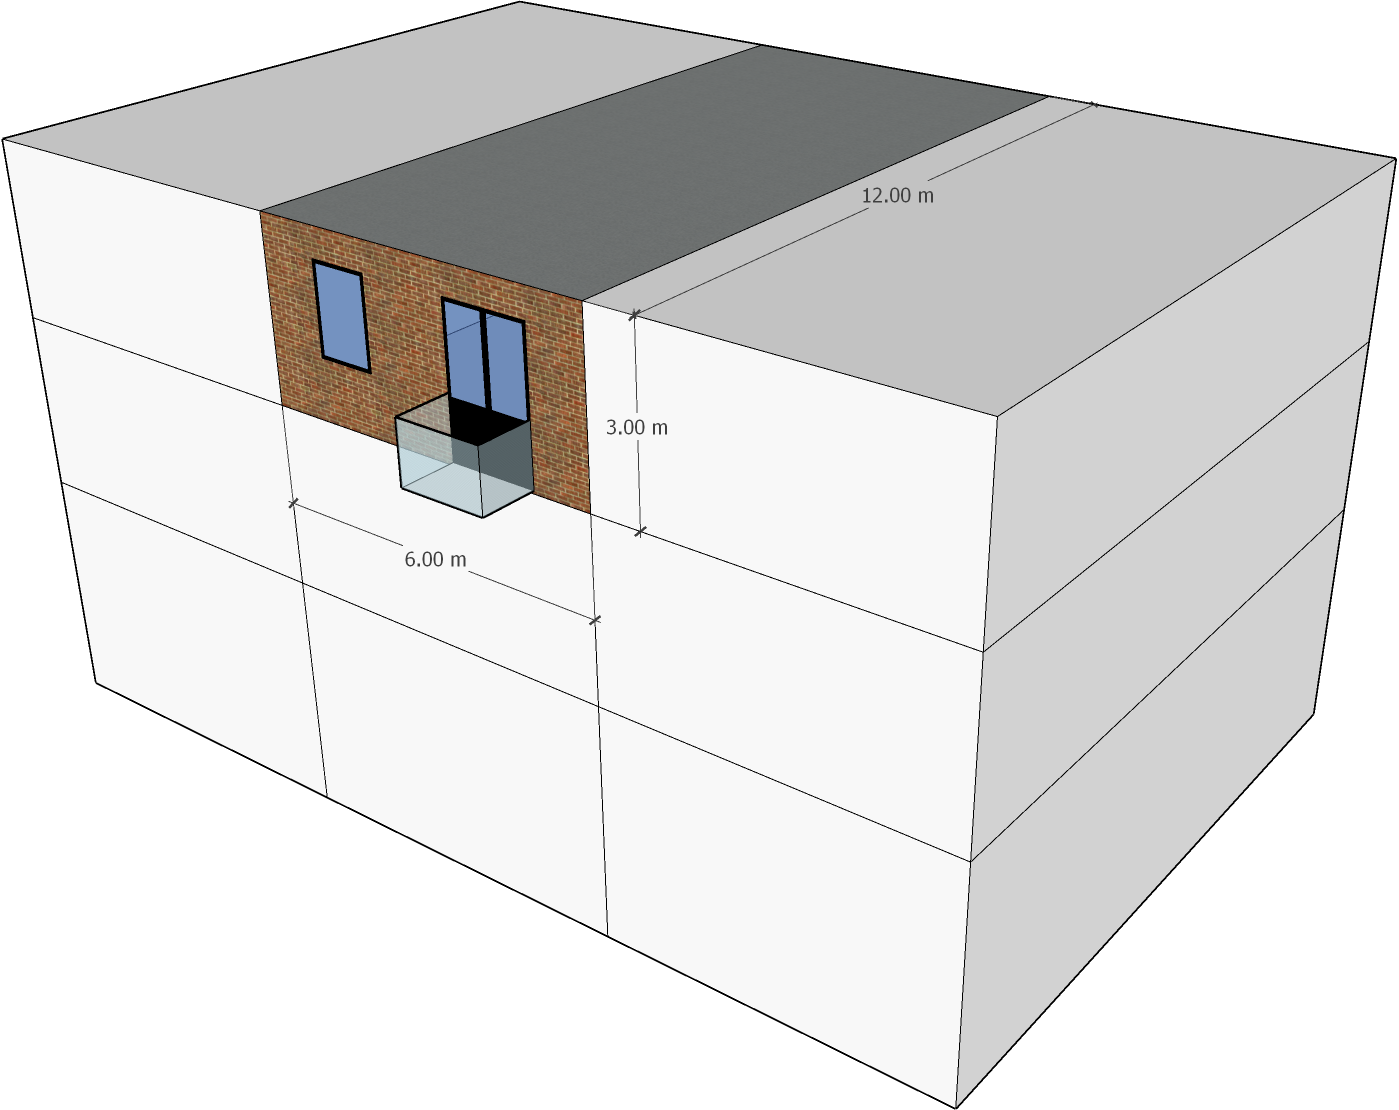
\includegraphics[height=9\baselineskip]{pictures/plex-unit}};


%\drawhelplines

% cooling results
\begin{groupplot}[group style={group size=1 by 3},
				  width=3\colvsep,
				  height=3\baselineskip,
				  xmin=0, xmax=48,
				  clip=false,
				  plot options,]

\nextgroupplot[
	axis x line=none,
	ymin=11.9, ymax=31.9,
	ytick={11.9, 31.9},
	yticklabels={11.9, \SI{31.9}{\celsius}},
	at={(p5cl cs:1,11)},
	anchor=south west,
	visible on=<2>]
\addplot[thick, col] table[x=time, y=TdbAmb] {data/case-study-cool.tsv};
\node[col, font=\footnotesize] at (axis cs:38,25) {\To};

\nextgroupplot[
	axis x line=none,
	ymin=14.898, ymax=26,
	ytick={14.9, 26},
	yticklabels={14.9, \SI{26}{\celsius}},
	at={(p5cl cs:1,7)},
	anchor=south west,
	visible on=<2>]
\addplot [gray!50] coordinates{(0,26) (48,26)};
\addplot [thick, gray] table[x=time, y=TdbSupply]
	{data/case-study-cool.tsv};
\addplot [thick,  col] table[x=time, y=TdbRoom] {data/case-study-cool.tsv};
\node [col, font=\footnotesize] at (axis cs:38,24) {\Tr};
\node [gray, font=\footnotesize] at (axis cs:38,16) {\Ts};


\nextgroupplot[
	xtick={0, 12, 17, 24, 31.25, 48},
	xticklabels={0:00, 12:00, \phantom{PM }5 PM, 0:00,
				 \phantom{AM }7:15 AM, 0:00},
	xticklabel style={name=ticklabel\ticknum},
	ymin=0, ymax=2.339,
	ytick={0, 1.1, 2.339},
	yticklabels={0, 1.1, \SI{2.3}{\kilo\watt}},
	at={(p5cl cs:1,3)},
	anchor=south west,
	visible on=<2>]
\addplot [thick, gray] table [x=time, y=QCoolSen]
	{data/case-study-cool.tsv};
\addplot [thick] table [x=time, y=PTot] {data/case-study-cool.tsv};
\addplot [thick, col] table [x=time, y=QCoolLat]
	{data/case-study-cool.tsv};
\node [gray, font=\footnotesize] at (axis cs:38,2) {\Qcs};
\node [col, font=\footnotesize] at (axis cs:38,0.8) {\Qcl};
\node [font=\footnotesize] at (axis cs:38,-.2) {\Pel};

\node [gray, anchor=west, yshift=-\baselineskip, font=\scriptsize] (day1)
	at (ticklabel0.west) {June 30, 2017};
\node [gray, anchor=west, yshift=-\baselineskip, font=\scriptsize]
	at (ticklabel3.west) {July 01, 2017};
\node [left, font=\scriptsize, inner sep=4\quanta]
	at (ticklabel0.west) {$t$};
\node [left, font=\scriptsize, inner sep=4\quanta] at (day1.west) {day};

\end{groupplot}



% heating results
\begin{groupplot}[group style={group size=1 by 3},
				  width=3\colvsep,
				  height=3\baselineskip,
				  xmin=0, xmax=48,
				  clip=false,
				  plot options,]

\nextgroupplot[
	axis x line=none,
	ymin=-17.9, ymax=7.771,
	ytick={-17.9, 7.771},
	yticklabels={\num{-17.9}, \SI{7.8}{\celsius}},
	at={(p5cl cs:1,11)}, anchor=south west,
	visible on=<3>]
\addplot[thick, col] table[x=time, y=TdbAmb] {data/case-study-heat.tsv};
\node[col, font=\footnotesize] at (axis cs:5,-1) {\To};

\nextgroupplot[
	axis x line=none,
	ymin=22, ymax=41.973,
	ytick={22, 41.973},
	yticklabels={22, \SI{42}{\celsius}},
	at={(p5cl cs:1,7)}, anchor=south west,
	visible on=<3>]
\addplot [gray!50] coordinates{(0,22) (48,22)};
\addplot [thick, gray] table[x=time, y=TdbSupply]
	{data/case-study-heat.tsv};
\addplot [thick,  col] table[x=time, y=TdbRoom] {data/case-study-heat.tsv};
\node [col, font=\footnotesize] at (axis cs:5,18) {\Tr};
\node [gray, font=\footnotesize] at (axis cs:5,32) {\Ts};


\nextgroupplot[
	xtick={0, 12, 20, 24, 36, 48},
	xticklabels={0:00, 12:00, 8 PM, 0:00, 12:00, 0:00},
	xticklabel style={name=ticklabel\ticknum},
	ymin=0, ymax=4.23,
	ytick={0, 4.23},
	yticklabels={0, \SI{4.2}{\kilo\watt}},
	at={(p5cl cs:1,3)}, anchor=south west,
	visible on=<3>]
\addplot [thick, gray] table [x=time, y=QHeat] {data/case-study-heat.tsv};
\addplot [thick, col] table [x=time, y=PTot] {data/case-study-heat.tsv};
\node[gray, font=\footnotesize] at (axis cs:5,2.1) {\Qh};
\node[col, font=\footnotesize] at (axis cs:5,-.6) {\Pel};

\node [gray, anchor=west, yshift=-\baselineskip, font=\scriptsize] (day1)
	at (ticklabel0.west) {Feb 10, 2017};
\node [gray, anchor=west, yshift=-\baselineskip, font=\scriptsize]
	at (ticklabel3.west) {Feb 11, 2017};
\node [left, font=\scriptsize, inner sep=4\quanta]
	at (ticklabel0.west) {$t$};
\node [left, font=\scriptsize, inner sep=4\quanta] at (day1.west) {day};

\end{groupplot}




% defrost detail
\begin{groupplot}[group style={group size=1 by 3},
				  width=3\colvsep,
				  height=3\baselineskip,
				  xmin=0, xmax=3,
				  clip=false,
				  plot options,]

\nextgroupplot[
	axis x line=none,
	ymin=-20, ymax=-18.4,
	ytick={-20, -18.4},
	yticklabels={\num{-20}, \SI{-18.4}{\celsius}},
	at={(p5cl cs:1,11)}, anchor=south west,
	visible on=<4>]
\addplot[thick, col] table[x=time, y=TdbAmb]
	{data/case-study-heat-detail.tsv};
\node[col, font=\footnotesize] at (axis cs:0.17,-19.4) {\To};

\nextgroupplot[
	axis x line=none,
	ymin=21.4, ymax=22.4,
	ytick={21.4, 22, 22.4},
	yticklabels={21.4, 22, \SI{22.4}{\celsius}},
	at={(p5cl cs:1,7)}, anchor=south west,
	visible on=<4>]
\addplot [gray!50] coordinates{(0,22) (3,22)};
\addplot [thick,  col] table[x=time, y=TdbRoom]
	{data/case-study-heat-detail.tsv};
\node [col, font=\footnotesize] at (axis cs:0.17,21.6) {\Tr};


\nextgroupplot[
	xtick={0, 3},
	xticklabels={7:00, 10:00},
	xticklabel style={name=ticklabel\ticknum},
	ymin=0, ymax=4.5,
	ytick={0, 3.228, 4.5},
	yticklabels={0, 3.2, \SI{4.5}{\kilo\watt}},
	at={(p5cl cs:1,3)}, anchor=south west,
	visible on=<4>]
\addplot [thick, gray] table [x=time, y=QHeat]
	{data/case-study-heat-detail.tsv};
\addplot [thick, col] table [x=time, y=PTot]
	{data/case-study-heat-detail.tsv};
\node[gray, font=\footnotesize] at (axis cs:0.17,5.2) {\Qh};
\node[col, font=\footnotesize] at (axis cs:0.17,2.4) {\Pel};

\node [gray, anchor=west, yshift=-\baselineskip, font=\scriptsize] (day1)
	at (ticklabel0.west) {Jan 12, 2017};
\node [left, font=\scriptsize, inner sep=4\quanta]
	at (ticklabel0.west) {$t$};
\node [left, font=\scriptsize, inner sep=4\quanta] at (day1.west) {day};

\end{groupplot}


\end{slide}



\section{}

% closing slide
\begin{maplayout}

\node[anchor=north east] at ($(page cs:44,11)+(0,0.4\baselineskip)$)
	{\includegraphics[height=2.8\baselineskip]{pictures/logo-poly.pdf}};
\node[anchor=base east] at (page cs:44, -11) {Gregor Strugala};
\node[anchor=base east] at (page cs:44, -27) {\color{gray} 22 mai 2019};

\end{maplayout}

\end{document}
